% Main Thesis File: This is the main file and it connects all the different parts of the thesis and compiles it into a single outcome file.

\documentclass[onecolumn, 12 pt, doublespace, fullpage, letterpaper, twoside, openright]{report}
\renewcommand{\baselinestretch}{1.75}

% Packages
\usepackage{float}
\usepackage{amssymb}
\usepackage{textcomp}
\usepackage{graphicx}
\usepackage{pdfpages}
\usepackage{graphics}
\usepackage{epsfig}
\usepackage{epstopdf}
\usepackage{float}
\usepackage{color}
\usepackage[cmex10]{amsmath}
\usepackage{latexsym,amsfonts}
\usepackage{amsthm}
\usepackage{url}
\usepackage{longtable}
\usepackage[figuresright]{rotating}
\usepackage{listings}
\usepackage{etoolbox}
\usepackage{emptypage}
\usepackage{titlesec}
\usepackage{natbib}
\usepackage{booktabs}
\usepackage[utf8]{inputenc}
\usepackage{pdflscape}
\usepackage{afterpage}
\usepackage{capt-of}% or use the larger `caption` package
\usepackage{siunitx}
\titleformat{\chapter}{}{}{0em}{\bf\Huge}
\titleformat{\section}{}{}{0em}{\bf\Large}
\setcounter{secnumdepth}{0}
\setcounter{tocdepth}{1}
\usepackage{fancyhdr}       
\pagestyle{fancy} 
\fancyhead{} \fancyfoot{} 
\fancyhead[CO,CE]{\thepage}      
\renewcommand{\headrulewidth}{0pt}


%The following code changes the empty vertical space above a new chapter title. It sets it from 50pt to 20pt
\makeatletter
\patchcmd{\@makechapterhead}{50\p@}{20pt}{}{}
\patchcmd{\@makeschapterhead}{50\p@}{20pt}{}{}
\makeatother
%end of modification



% The following code redefines the plain pagestyle with the objective of moving the page number from the bottom to the top of the page. This only affects new chapter pages.
\fancypagestyle{plain}{
\fancyhf{} %clear all header and footer fields
\fancyhead[C]{\thepage} %puts number on top center of the page
\renewcommand{\headrulewidth}{0pt}
\renewcommand{\footrulewidth}{0pt}}
%ending of plain pagestyle modification.


\usepackage{setspace}
\usepackage{subfigure}

% ### Nomenclature, List of Abbreviations and List of Symbols 
   \usepackage{ifthen,xkeyval,xfor,amsgen}
   \usepackage[acronym,toc]{glossaries}
   \newglossary[slg]{symbols}{syi}{sbl}{List of Symbols}
   \makeglossaries
   
   
% #### Symbols ####
\newglossaryentry{symb:Pi}{
name=$\pi$, type=symbols,
description=A mathematical constant whose value is the ratio of any circle's circumference to its diameter,
sort=symbolpi
}

\newglossaryentry{symb:Phi}{
name=$\varphi$, type=symbols,
description=An angle,
sort=symbolphi
}

\newglossaryentry{symb:Lambda}{
name=$\lambda$, type=symbols,
description={Lambda indicates usually an eigenvalue in linear algebra},
sort=symbollambda
}

% #### Abbreviations ####
\newacronym{toc}{ToC}{Table of Contents}
\newacronym{los}{LoS}{List of Symbols}
\newacronym{loa}{LoA}{List of Abbreviations}
\newacronym{phd}{PhD}{Doctoral}
\newacronym{MS}{MS}{Masters}
\newacronym{M$}{MS}{Microsoft}
\newacronym{CD}{CD}{Compact Disc}
\newacronym{kaust}{KAUST}{King Abdullah University of Science and Technology}

%An acronym with a glossary entry
\newacronym{AD}{AD}{Active Directory\protect\glsadd{glos:AD}}



% #### Nomenclature terms ####
\newglossaryentry{glos:AD}{
name=Active Directory,
description={Active Directory is the directory service for Windows based networks, that allows central organization and administration of any network resource. It allows a single-sign-on concept independent from network topologies or network protocols. As a prerequisite you need a Windows Server acting as Domain Controller. This computer stores all necessary data, e.g.~usernames and corresponding passwords}
}

\newglossaryentry{glos:RespF}{name=response file, description={A file 
that allows unattended software installation}}


   % Run the following three lines in the command line to get the lists
%makeindex -s Thesis.ist -t Thesis.alg -o Thesis.acr Thesis.acn
%makeindex -s Thesis.ist -t Thesis.slg -o Thesis.syi Thesis.sbl
%makeindex -s Thesis.ist -t Thesis.glg -o Thesis.gls Thesis.glo

% ### End of addition

\usepackage{hyperref} 


% Modified commands
\newcommand{\Tab}{\hspace{2ex}}
\usepackage[lmargin=1.5in, rmargin=1in, vmargin=1in, headsep=0.083334in]{geometry}
\newcommand{\mathsym}[1]{{}}
\newcommand{\unicode}[1]{{}}
\renewcommand{\thechapter}{\arabic{chapter}}
\renewcommand\bibname{\centering BIBLIOGRAPHY}

\pagenumbering{roman}
\begin{document}

%\raggedright %to make the text left aligned.

\vspace{2pt}
\thispagestyle{empty}
\addvspace{10mm}

\begin{center}
{\bf\Large Data-Driven and Dynamics-Driven Approaches for Forecasting the Red Sea Chlorophyll}\vfill
{\Large Thesis by}\\
{\bf\Large Denis Dreano}\vfill
{\Large In Partial Fulfillment of the Requirements}\\[12pt]
{\Large For the Degree of}\\[12pt]
{\bf\Large Doctor of Philosophy} \vfill
{King Abdullah University of Science and Technology, Thuwal,}\\
{Kingdom of Saudi Arabia}
\vfill
%\maketitle
{Insert Date (Month, Year)}\vfill

\end{center}

\newpage
\noindent{The thesis of Your Full Name is approved by the examination committee}
% \addcontentsline{toc}{chapter}{Examination Committee Approval}

\vspace{6\baselineskip}

\noindent{Committee Chairperson: Your advisor's name}\\
Committee Member: Second name\\
Committee Member: Third name\vfill

%\begin{center}
%{King Abdullah University of Science and Technology}\\
%{Year}
%\end{center}

\newpage
% \addcontentsline{toc}{chapter}{Copyright}
\vspace*{\fill}
\begin{center}
{Copyright \copyright Year}\\
{Your Full Name}\\
{All Rights Reserved}
\end{center}


\begin{onehalfspacing}%To make the table of contents, figures, and tables single spaced, as required by the formatting guidelines, pg. 24.
\renewcommand{\contentsname}{\centerline{TABLE OF CONTENTS}}
\tableofcontents
\cleardoublepage

% \printglossary[type=\acronymtype,style=long3col, title=\centerline{LIST OF ABBREVIATIONS}, toctitle=List of Abbreviations, nonumberlist=true] 
% \printglossary[type=symbols,style=long3col, title=\centerline{LIST OF SYMBOLS}, toctitle=List of Symbols, nonumberlist=true] 
% 
% \cleardoublepage
% \addcontentsline{toc}{chapter}{\listfigurename} 
% \renewcommand*\listfigurename{\centerline{LIST OF FIGURES}} 
% \listoffigures
% 
% \cleardoublepage
% \addcontentsline{toc}{chapter}{\listtablename}
% \renewcommand*\listtablename{\centerline{LIST OF TABLES}} 
% \listoftables

\end{onehalfspacing}
% \printglossary[style=altlist,title=Nomenclature, toctitle=Nomenclature, nonumberlist=true] 

% <Old plan>
%
% Thesis Introduction File

\chapter{Motivation}

\section{Importance of phytoplankton}

Phytoplankton are unicellular, photosynthetic algae that live in the upper layers of bodies of water (ocean, lakes, rivers or ponds). There a three main types of phytoplankton species: diatom (5-200μm), dinoflagellates (5-200μm) and cyanobacteria (<5μm). Diatoms and dinoflagellates are found in nutrient rich environments and multiply rapidly when conditions are favorable. On the other hand, cyanobacteria are capable of surviving in very oligotrophic (nutrient poor) environments like the Red Sea. In the oceans, phytoplankton live in the surface layer where there is enough sunlight for photosynthesis. 

Phytoplankton plays a fundamental role for the ocean ecology as it is at the basis of the marine food web. Zooplankton graze phytoplankton which are consumed by larger species. Higher concentrations of phytoplankton will therefore result in larger stock of predator fishes. High phytoplankton concentration also impact their environment by creating dead zone when they die and are decomposed by bacteria. Due to the rapid growth of phytoplankton, it responds very well to changes in its environment, making it a key parameter to monitor the water quality.

Due to phytoplankton place at the bottom of the marine food chain, it is a key factor for fisheries and the marine ecology. Productive fishing zones like the regions in the Arabian seas, Californian coast, north-west African coast and Chilean coast are explained by the upwelling of cold nutrient rich water favourable to phytoplankton, which in turn feeds higher trophic levels. On the other hand, during the El-Nino phenomenon creates less favourable conditions for phytoplankton in the Eastern Pacific, resulting in a dramatic reduction of fish catches of fisheries in the western coast of South America.

Phytoplankton also plays the role of a biological CO2 pump and strongly impact the Earth climate. During photosynthesis, phytoplankton captures carbon and releases oxygen. A part of this organic material stays in the food web, either transmitted to higher trophic level, or degraded  by bacteria. Another part however sinks to the bottom of the ocean and sediments. Research is currently done to evaluate the way this biological pump works and how it affects climate. 

\section{Measuring Chlorophyll Concentration}

Chlorophyll is a molecule that is food in algae, phytoplankton and plants that is critical for photosynthesis. Phytoplankton is a poor absorber of green light, and is responsible for the coloration of plants. When phytoplankton are present in high concentrations they change the water also takes a detectable green coloration (it can also take a red or blue coloration depending on the type of phytoplankton dominating). This offers a way to estimate the chlorophyll concentration of the water, which is a good proxy for phytoplankton concentration. 

In-situ measurements of chlorophyll are however expensive and have limited temporal and spatial coverage. In-situ measurement of chlorophyll concentration can be gathered through scientific cruises, buoy stations or gliders (unmanned submarines). These methods are expensive to deploy and therefore the coverage is limited. Political issues, like in the Red Sea, can also be a practical barrier to in-situ measurements. 

Satellite measurements of chlorophyll provide excellent proxies for phytoplankton concentrations with a good temporal and spatial coverage. The SeaWIFS, MODIS and MERIS missions have provided an uninterrupted coverage of the world since 1997. High-resolution maps of daily chlorophyll concentration are freely accessible to the scientific community. Despite some limitations, in particular of missing data due to cloud coverage and sunglint, or problematic values in coastal areas, remotely-sensed chlorophyll concentration are used intensively by the scientific community. In regions, like in the Red Sea, where little in-situ measurements are available, it is often the most important data source. 

\section{Primary productivity in the Red Sea}

Typical tropical seas (TTS), like the Red Sea, are characterized by a highly stratified structure, where warm nutrient-depleted surface water is separated by cold nutrient-rich by a steep gradient of temperature zone called pycnocline. The pycnocline acts as barrier that prevents nutrients to reach the surface water. As a result, TTS are oligotrophic and have low chlorophyll concentrations. Until recently, marine biologists have thought that TTS had therefore a very low productivity. However, recent investigations have contested this idea, that different upwelling mechanisms exist that bring new nutrients to the surface water. 

Despite being an oligotrophic and challenging environments for marine life, the Red Sea presents a surprisingly rich and diverse ecosystem. Most of it lives in the very developed coral reef system. The source of nutrient for sustaining such a developed ecosystem is not well understood yet, but the interaction with the open sea through the mesoscale eddies is believed to play an important role. 

Remotely-sensed chlorophyll data show an important seasonality of the Red Sea primary productivity, that has been linked to winter deep mixing, and the inversion of the wind direction in the southern Red Sea, enhancing intrusion of nutrient rich Gulf of Aden water. Despite this strong seasonality, there is a large interannual variability caused by the unpredictable occurrence of large phytoplanktonic blooms. Diverse causes have been hypothesized for these blooms such as wind-induced mixing, eddies or dust storms carrying nutrients. 

Although the Red Sea environment is relatively preserved, it is under increasing pressure due to human activities. An abrupt increase of temperature has occurred in the last decade that threatens the fragile coral reef system. Moreover, the increasing urbanization and fishing activity contribute to the fragilization of this unique ecosystem.

\section{Chlorophyll Concentration Prediction}

Models can be useful to identify causes behind the chlorophyll patterns we observe in the Red Sea. Many hypotheses have be made about the drivers of chlorophyll concentration in this regions, but some of them have not been yet investigated through models. The role played by the exchange of water with the Gulf of Aden and winter overturning in the northern Red Sea have been successfully modeled with circulation and ecological models. However, the interaction between the open sea and coral reefs and the role of sand storms has not been investigated yet. Models, can also be helpful in discovering new dynamics affecting the chlorophyll concentration. In particular, the interaction between the productivity level of the different regions of the Red Sea has not been studied yet.  

Model predictions for chlorophyll concentration can also have practical applications. Phytoplankton blooms can be harmful to humans and marine life and are closely monitored in many regions of the world. In the Red Sea, where tourism and aquaculture are developing it is likely to become a concern too. Phytoplankton is also directly, and indirectly through zooplankton, the cause of microfouling that affects desalination plants. Anticipating a phytoplanktonic bloom might therefore be helpful in taking preventive actions. Finally, due to their short life-cycle, phytoplankton concentration reacts quickly to changes the environment, making it a  key variable in water quality monitoring.

\section{Modeling Chlorophyll Concentration}

Ecological ordinary differential equation (ODE) deterministic models are a popular way to model marine ecology. Such models can be as simple as the nutrient-phytoplankton-zooplankton (NPZ) model that only has three variables representing two trophic level, or as complex as the European regional seas ecosystem model (ERSEM) that has dozens of variables and represent many ecological, biological and chemical interactions. Such a model has been couple to the MITgcm circulation model used to simulate the Red Sea ecology. However the complexity of these models makes them difficult to deploy and interpret their results. 

On the other hand, data-driven statistical models are relatively easier to apply. They are relevant when the phenomenon producing the data is very complex or poorly known. They have been applied to predict chlorophyll concentration, mostly in small regions that have complex dynamics. Some statistical models, such as linear regression, GAM or tree regression have the advantage of being easy to interpret, and can be used to understand the dynamics driving the chlorophyll concentration.

Phenomena such as propagation and diffusion play a key role in the chlorophyll spatial concentration, but are difficult to represent without spatial modeling. There is also a difference in the chlorophyll patterns of different regions of the Red Sea, in particular between the nutrient rich southern Red Sea and the oligotrophic northern Red Sea, and between the open ocean and the coastal waters. There is however no clear cut division between regions with different pattern, making it difficult to divide the Red Sea into regions. Finally the different regions of the Red Sea are believed to interact. A model is therefore needed to account for the spatial and temporal interaction of the chlorophyll.

Classical geostatistics is the most widely used spatial statistical models. It models spatial data as the realization of a two dimensional Gaussian process, of which one can estimate the parameters. Geostatistics can be easily extended to spatio-temporal datasets. Many flexible ways of constructing space-time covariance functions for these models have been proposed recently. Space-time geostatistics has been applied to many environment studies, but not to chlorophyll data yet.


%
% Thesis Introduction File

\chapter{Motivation}

\section{Importance of phytoplankton}

Phytoplankton are unicellular, free-floating, photosynthetic algae that live in the upper layers of bodies of water (ocean, lakes, rivers or ponds). There exists a wide diversity of phytoplankton species. To this date, about 5000 of them have been identified \cite{Tett1995}. Phytoplankton are also highly variable in sizes, ranging from 0.2μm for cyanobacteria to 200μm for the largest species of diatom \cite{Pal2014}. In the oceans, phytoplankton live in the surface layer where there is enough sunlight for photosynthesis. 

Phytoplankton plays a fundamental role for the ocean ecology. It is the basis of the marine food web and traps most of the energy used by pelagic ecosystems \cite{Pal2014}. Zooplankton graze phytoplankton which are then consumed by higher trophic levels. It has been estimated that nearly 98\% of the ocean primary productivity comes from phytoplankton \cite{Pal2014}. Phytoplankton are also responsible for maintaining the dissolved oxygen level necessary for other species to survive. However, high phytoplankton concentration also impact their environment by creating dead zone when they die and are decomposed by bacteria, consuming all the available oxygen \cite{Pal2014}. Due to the rapid growth of phytoplankton, it responds very well to changes in its environment, making it a key parameter to monitor the water quality \cite{Wu2014}.

Due to phytoplankton place at the bottom of the marine food chain, it is a key factor for fisheries. Productive fishing zones like the regions in the Arabian seas, Californian coast, north-west African coast and Chilean coast are explained by the upwelling of cold nutrient rich water favourable to phytoplankton, which in turn feeds higher trophic levels. On the other hand, during the El-Nino phenomenon creates less favourable conditions for phytoplankton in the Eastern Pacific, resulting in a dramatic reduction of fish catches of fisheries in the western coast of South America \cite{Robinson2010}. Remotely-sensed chlorophyll data have been routinely used since the past decades to help fisheries predict the timing phytoplankton blooms \cite{Robinson2010}

Phytoplankton also plays the role of a biological CO2 pump and strongly impact the Earth climate. During photosynthesis, phytoplankton captures carbon and releases oxygen. A part of this organic material stays in the food web, either transmitted to higher trophic level, or degraded  by bacteria. Another part, however, sinks to the bottom of the ocean and sediments. It is estimated that phytoplankton account for 48\% of Earth carbon fixation \cite{Pal2014}.

\section{Measuring Chlorophyll Concentration}

Chlorophyll is a molecule that is food in algae, phytoplankton and plants that is critical for photosynthesis. Phytoplankton is a poor absorber of green light, and is responsible for the coloration of plants. When phytoplankton are present in high concentrations they change the water also takes a detectable green coloration (it can also take a red or blue coloration depending on the type of phytoplankton dominating). This offers a way to estimate the chlorophyll concentration of the water, which is a good proxy for phytoplankton concentration. 

In-situ measurements of chlorophyll are however expensive and have limited temporal and spatial coverage. In-situ measurement of chlorophyll concentration can be gathered through scientific cruises, buoy stations or gliders (unmanned submarines). These methods are expensive to deploy and therefore the coverage is limited. Political issues, like in the Red Sea, can also be a practical barrier to in-situ measurements. 

Satellite measurements of chlorophyll provide excellent proxies for phytoplankton concentrations with a good temporal and spatial coverage. The SeaWIFS, MODIS and MERIS missions have provided an uninterrupted coverage of the world since 1997. High-resolution maps of daily chlorophyll concentration are freely accessible to the scientific community. Despite some limitations, in particular of missing data due to cloud coverage and sunglint, or problematic values in coastal areas, remotely-sensed chlorophyll concentration are used intensively by the scientific community. In regions, like in the Red Sea, where little in-situ measurements are available, it is often the most important data source. 

\section{Primary productivity in the Red Sea}

Typical tropical seas (TTS), like the Red Sea, are characterized by a highly stratified structure, where warm nutrient-depleted surface water is separated by cold nutrient-rich by a steep gradient of temperature zone called pycnocline. The pycnocline acts as barrier that prevents nutrients to reach the surface water. As a result, TTS are oligotrophic and have low chlorophyll concentrations. Until recently, marine biologists have thought that TTS had therefore a very low productivity. However, recent investigations have contested this idea, that different upwelling mechanisms exist that bring new nutrients to the surface water. 

Despite being an oligotrophic and challenging environments for marine life, the Red Sea presents a surprisingly rich and diverse ecosystem. Most of it lives in the very developed coral reef system. The source of nutrient for sustaining such a developed ecosystem is not well understood yet, but the interaction with the open sea through the mesoscale eddies is believed to play an important role. 

Remotely-sensed chlorophyll data show an important seasonality of the Red Sea primary productivity, that has been linked to winter deep mixing, and the inversion of the wind direction in the southern Red Sea, enhancing intrusion of nutrient rich Gulf of Aden water. Despite this strong seasonality, there is a large interannual variability caused by the unpredictable occurrence of large phytoplanktonic blooms. Diverse causes have been hypothesized for these blooms such as wind-induced mixing, eddies or dust storms carrying nutrients. 

Although the Red Sea environment is relatively preserved, it is under increasing pressure due to human activities. An abrupt increase of temperature has occurred in the last decade that threatens the fragile coral reef system. Moreover, the increasing urbanization and fishing activity contribute to the fragilization of this unique ecosystem.

\section{Chlorophyll Concentration Prediction}

Models can be useful to identify causes behind the chlorophyll patterns we observe in the Red Sea. Many hypotheses have be made about the drivers of chlorophyll concentration in this regions, but some of them have not been yet investigated through models. The role played by the exchange of water with the Gulf of Aden and winter overturning in the northern Red Sea have been successfully modeled with circulation and ecological models. However, the interaction between the open sea and coral reefs and the role of sand storms has not been investigated yet. Models, can also be helpful in discovering new dynamics affecting the chlorophyll concentration. In particular, the interaction between the productivity level of the different regions of the Red Sea has not been studied yet.  

Model predictions for chlorophyll concentration can also have practical applications. Phytoplankton blooms can be harmful to humans and marine life and are closely monitored in many regions of the world. In the Red Sea, where tourism and aquaculture are developing it is likely to become a concern too. Phytoplankton is also directly, and indirectly through zooplankton, the cause of microfouling that affects desalination plants. Anticipating a phytoplanktonic bloom might therefore be helpful in taking preventive actions. Finally, due to their short life-cycle, phytoplankton concentration reacts quickly to changes the environment, making it a  key variable in water quality monitoring.

\section{Modeling Chlorophyll Concentration}

Ecological ordinary differential equation (ODE) deterministic models are a popular way to model marine ecology. Such models can be as simple as the nutrient-phytoplankton-zooplankton (NPZ) model that only has three variables representing two trophic level, or as complex as the European regional seas ecosystem model (ERSEM) that has dozens of variables and represent many ecological, biological and chemical interactions. Such a model has been couple to the MITgcm circulation model used to simulate the Red Sea ecology. However the complexity of these models makes them difficult to deploy and interpret their results. 

On the other hand, data-driven statistical models are relatively easier to apply. They are relevant when the phenomenon producing the data is very complex or poorly known. They have been applied to predict chlorophyll concentration, mostly in small regions that have complex dynamics. Some statistical models, such as linear regression, GAM or tree regression have the advantage of being easy to interpret, and can be used to understand the dynamics driving the chlorophyll concentration.

Phenomena such as propagation and diffusion play a key role in the chlorophyll spatial concentration, but are difficult to represent without spatial modeling. There is also a difference in the chlorophyll patterns of different regions of the Red Sea, in particular between the nutrient rich southern Red Sea and the oligotrophic northern Red Sea, and between the open ocean and the coastal waters. There is however no clear cut division between regions with different pattern, making it difficult to divide the Red Sea into regions. Finally the different regions of the Red Sea are believed to interact. A model is therefore needed to account for the spatial and temporal interaction of the chlorophyll.

Classical geostatistics is the most widely used spatial statistical models. It models spatial data as the realization of a two dimensional Gaussian process, of which one can estimate the parameters. Geostatistics can be easily extended to spatio-temporal datasets. Many flexible ways of constructing space-time covariance functions for these models have been proposed recently. Space-time geostatistics has been applied to many environment studies, but not to chlorophyll data yet.



%\chapter{Objectives}

The goal of the dissertation is to show that statistical predictive models can be used to help efficiently forecasting chlorophyll concentration in the Red Sea. Statistical methods can be more robust and computationally efficient when the underlying dynamics are very complex and observations are limited. The study of chlorophyll concentration is such a case. The dissertation will compare the 8-days prediction skill of increasingly sophisticated predictive models to the highly sophisticated ecological model ERSEM. We will explore the possibilities of combining statistical and deterministic models to improve the chlorophyll forecasts.

Efficient statistical models may be used as alternatives to the much more complex deterministic models in other seas. They can help researchers to gain insight into the dynamics of the phytoplankton. They can also help coastal communities to mitigate the effects of harmful phytoplankton blooms on public health and their economy. Moreover this study will help confirming hypothesizes that have been made about the interaction of Red Sea phytoplankton with the regional and global circulation. 


%\section{Task 1: Dataset building and Exploration}

\noindent
\emph{Duration: 2 months (by December 2014)}

\noindent
\emph{Submission: Journal of Marine Systems}

\noindent
\emph{Collaborator: Dionysios Raitsos}

\subsection{Motivation}

A preliminary task to data modeling, is the gathering, cleaning and exploration of the data. Given the complexity and the size (40 GB) of the data, this is not an easy task. This first data analysis, will reveal if enough data has been gathered to make meaningful forecast, and what accuracy we can expect from the models. This step will also provide information that will help in designing statistical models: most significant variables, differences between regions, relevant data transformation, etc. Finally, this step will identify patterns in the data that will be useful to qualitatively evaluate predictive models.

\subsection{Open Questions}

\begin{itemize}
\item Can we efficiently identify outliers in the chlorophyll values?
\item Is there a way to efficiently fill the missing values in the chlorophyll dataset?
\item Can the data help understanding the mechanisms behind extreme blooms in the Red Sea?
\item Can the hypothesizes about the dynamics behind the chlorophyll seasonal cycle be confirmed by the data?
\item Are there more blooms in the past years?
\end{itemize}

\subsection{Method and Work Done}

\begin{enumerate}
\item Identify data sources and load the data…………………………………………………60%
\item Clean the data and fill missing values (DINEOF)......................................................50%
\item Align and format the data in order to have a unique dataset…………………………...0%
\item Explore the dataset………………………………………………………………………..20%
\begin{itemize}
\item Study the correlation between chlorophyll and other variables (Linear Regression, GAM, data transformations)
\item Select variables (Lasso, single variable regression, multistep regression)
\item Study the regional aggregation (ACF)
\item Explore spatiotemporal correlations (hovmoller plots, PCA, variograms)
\item Estimate the Bayes factor/ % of variance explained (k-nearest neighbors)
\end{itemize}
\end{enumerate}

\subsection{Expected Outcomes}

\begin{itemize}
\item A cleaned dataset that can be used in the following tasks
\item A comprehensive exploration of the available data for chlorophyll study in the Red Sea
\item A preliminary variable selection
\item A clear picture of the major spatio-temporal patterns in the data
\item A critical evaluation of the current hypothesis about the chlorophyll dynamics in the Red Sea
\end{itemize}

\subsection{Work Accomplished and Prelimnary results}

%\section{Chapter 2: Forecasting Chlorophyll Concentration in Regional Aggregates}

\noindent
\emph{Duration: 2 months (by February 2015)}

\noindent
\emph{Submission: Progress in Oceanography}

\noindent
\emph{Collaborator: Dionysios Raitsos}

\paragraph{Motivation}

Chlorophyll data is very complex. It is therefore useful to first simplify it by aggregating it spatially. The space-time dynamics of the chlorophyll data reflects the highly nonlinear dynamics of the underlying physical, chemical and biological phenomenons. As shown by the north-south gradient and the seasonal behavior, the resulting space-time process is nonstationary in time and in space. The high-dimensionality in space can be reduced by considering a regional aggregation of the results. This would allow us to focus on the global scale phenomenons: such as the interactions between neighboring regions, the time-scale of large events and the difference in the physical variables affecting the chlorophyll concentration in each region. In the following tasks, these simple predictive models will also be a reference for evaluating more complex ones. 

\paragraph{Open Questions}

\begin{itemize}
\item Is the biological aggregation of the Red Sea proposed by (Raitsos 2013) statistically meaningful?
\item Can clustering methods be used to identify marine ecological zones based on chlorophyll data?
\item Can a simple forecasting model allow us to understand the causes of chlorophyll blooms?
\item Can the current hypothesizes about the seasonal chlorophyll dynamics be validated?
\end{itemize}

\paragraph{Method}

\begin{enumerate}
\item Define datasets (training and test datasets, cross-validation).....................................0%
\item Variable selection (Lasso, L1 regression, single-variable linear regression)...............0%
\item Define regional aggregations (unsupervised learning, Hierarchical clustering, K-means)...................................................................................................................50%
\item Forecasts chlorophyll concentration (linear regression, GAM models, diagnostic, k-nearest neighbors)....................................................................................................0%
\item Predicting future extreme blooms (nearest-neighbours, logistic regression, decision trees)...........................................................................................................................0%
\end{enumerate}

\paragraph{Expected Outcomes}

\begin{itemize}
\item A regional division of the Red Sea that has been quantitatively evaluated.
\item A critic of current hypothesis about the chlorophyll dynamics in the Red Sea.
\item A lower bound on the performance of a more sophisticated model.
\item An assessment of the limitation of aggregate methods for Chlorophyll data.
\item An understanding on how the treatment of spatial correlations can improve the results.
\end{itemize}

\paragraph{Work Accomplished and Prelimnary results}

%\section{Chapter 3: Global geostatistical model for forecasting}

\noindent
\emph{Duration: 1 month (by March 2015)}

\noindent
\emph{Submission: Spatial Statistics}

\paragraph{Motivation}

Geostatistical methods can be used to construct dynamical models for forecasting the chlorophyll concentrations that we can compare to deterministic models. Geostatistics is a robust method to model spatio-temporal data. Recently there has been a lot of research on expanding it to model spatio-temporal data. With Kriging, these models a are powerful ways to do spatio-temporal prediction. As a particular case of Kriging, by predicting the spatial future field given the observation of the present field, we can derive a linear dynamical model. This linear model can be employed in a filtering setting like the Kalman filter. This is a desirable setup, as it is similar to the way deterministic models are employed to do forecasts given past observations. 

\paragraph{Open Questions}

\begin{itemize}
\item Can a global geostatistical model fit chlorophyll data?
\item How non stationary is the data in time and space?
\item What spatiotemporal covariance functions best fit the chlorophyll data?
\item Can geostatistical methods be employed in a filtering setup?
\end{itemize}

\paragraph{Method}

This task has already been started and had been the object of a submission for publication. The remaining work includes:
Use the new dataset and the new covariates
Compare the results to the ones of with the regional aggregates
Expected Outcomes
A methodology to employ a geostatistical model in a filtering problem.
A characterization of the space-time non stationarity of the data, and the interaction of the temporal and spatial dimensions.
An understanding of how spatial aggregation and geostatistical models can be used in the same model. 

\paragraph{Work Accomplished and Preliminary Results}



%\section{Task 4: Local geostatistical model for forecasting}

\noindent
\emph{Duration: 3 months (by June 2015)}

\noindent
\emph{Submission: Journal of the American Statistical Association (Case Study)}

\noindent
\emph{Collaborator: Raphael Huser}

\subsection{Motivation}

This part will bring together the results of the two preceding tasks to develop a predictive model that takes into account the large-scale dynamics and the regional spatio-temporal dynamics. In task 2, a predictive model is built, that represents the large scales behaviour of the Red Sea, but the spatial dimension inside each region is not addressed. We expect local features to play a role, such as the proximity to the coast, the bathymetry, proximity to other regions or major cities, etc. In task 3, we developed a methodology to use a geostatistical model in a dynamic fashion to do pixel-scale forecast. In this task, each regions will be modeled separately by a local geostatistical model that can do local prediction. These models will have access to aggregate covariates from neighboring regions in represent the global scale behaviours. 

\subsection{Open Questions}

\begin{itemize}
\item What are the most adapted space-time covariance models for chlorophyll data?
\item How to use global covariates in a geostatistical model?
\item What are the differences in the fine-scale dynamics of chlorophyll in each region?
\item Can the fine scale behaviour of phytoplankton be predicted accurately?
\item What are the spatial features that are important for the chlorophyll dynamics?
\end{itemize}

\subsection{Method}

\begin{itemize}
\item Extract local dataset from previous tasks
\item Design the training and test datasets, and the cross-validation method
\item Design and evaluate the mean function given the past covariates
\item Fit the local geostatistical model to the residuals.
\item Evaluate the model predictions and compare the results with task 2 and 3.
\end{itemize}

\subsection{Expected Outcomes}

\begin{itemize}
\item A methodology to aggregate local geostatistical models
\item An improvements in the prediction skills over the models of task 2 and 3.
\item An understanding of the differences between each regions.
\item A critical evaluation of the space-time covariance models for fitting chlorophyll data.
\item A better characterization of the regional chlorophyll dynamics.
\end{itemize}

%\section{Chapter 5: Assimilation of 1D ecological models and comparison to statistical models}

\noindent
\emph{Duration: 3 months (by September 2015)}

\noindent
\emph{Submission: Journal of Geophysical Research}

\noindent
\emph{Collaborator: George Triantafyllou / Boujeema}

\paragraph{Motivation}

The three previous tasks focus on constructing increasingly sophisticated predictive models for the chlorophyll concentration in the Red Sea. In this part these models will be compared to a 1D ecological model (ERSEM). This model is well detailed and very complex. The goal of this part will be to identify the merits of each modeling approach, and propose ways in which they can complement each other. To allow for comparison, the model will be run in each of the regions found in task 2. Available data will also be assimilated to the model through a smoothing assimilation scheme that will use an expectation-maximization algorithm for parameters estimation. 

\paragraph{Open Questions}

\begin{itemize}
\item Are statistical methods competitive for forecasting chlorophyll concentrations?
\item How can statistical and deterministic models complements each other?
\item Can statistical method forecast interesting dynamical features?
\item Are there significant regional differences in the relative performances of both approaches?
\item How to estimate the parameters of ecological models? 
\end{itemize}

\paragraph{Method}

\begin{enumerate}
\item Define the metrics for comparison
\item Calibrate the ERSEM model on each of the regions
\item Define an assimilation scheme and the data for the ERSEM model
\item Implement the assimilation scheme
\item Run the simulation and aggregate the results
\item Do the comparisons with the statistical models
\end{enumerate}

\paragraph{Expected Outcomes}

\begin{itemize}
\item A complete set of measures of the prediction skills of each approach.
\item A method to estimate assimilation and model parameters in an assimilated ecological model.
\item A set of case studies of the behaviours of each method for forecasting interesting events.
\item An understanding of the limitations of geostatistical models to predict nonlinear dynamics. 
\item Propositions on how the two approaches can complement each other.
\end{itemize}

\paragraph{Work Accomplished and Preliminary Results}


%\section{Task 6: Improving an Ecological Model Data Assimilation Scheme through Statistical Predictive Models}

\noindent
\emph{Duration: 3 months (by September 2015)}

\noindent
\emph{Submission: Journal of Geophysical Research}

\noindent
\emph{Collaborator: George Triantafyllou / Boujeema}

\section{Motivation}

In the previous task, we compared the forecasts of the ecological ERSEM model to that of the statistical models we developed from tasks 2 to 4. In this task we will study how these two approaches can be complementary. Specifically, we will study the use of statistical forecasts model to improve the forecasts of the ERSEM ecological model. The forecasts of the statistical models will be treated as observations, that can be assimilated by the filtering scheme used with the ERSEM model, and will give an improved forecast. When real observations will be available, they will be assimilated sequentially. This, method will allow the different ERSEM models on each cluster to communicate indirectly their states to one another. 

\subsection{Open Questions}

\begin{itemize}
\item Can statistical predictive models be used to communicate information between deterministic model?
\item Would the access to information about other regions improve the model forecasts?
\item What are the global patterns of ecological dynamics in the Red Sea?
\end{itemize}

\subsection{Method}

\begin{enumerate}
\item Define new assimilation scheme
\item Define metrics to measure model improvement
\item Prepare training and test datasets
\item Train statistical model
\item Run simulation with assimilation of statistical observation
\item Compare with results of task 5
\end{enumerate}

\subsection{Expected Outcomes}

\begin{itemize}
\item An improvement in the prediction skills of the deterministic approach
\item A methodology to couple deterministic ecological models through statistical models
\item Insights on the global ecological dynamics of the Red Sea
\end{itemize}



%\chapter{Literature Review}

\section{Red Sea large-scale phytoplankton dynamics}

Despite an increasing number of study for the last two decades, the large-scale phytoplankton dynamics of the Red Sea remains largely unknown \cite{Raitsos2013, Triantafyllou2014}. The Red Sea is deficient in the major nutrients \cite{Weikert1987}, and the only significant input of fresh water comes from the Gulf of Aden. This explains a general increase of chlorophyll concentration from north to south with the NCRS having the lowest concentration \cite{Raitsos2013}. The Red Sea also displays a distinct seasonality, with the highest chlorophyll concentration in winter. A minor summer peak is also observed around July, everywhere except in the NRS \cite{Raitsos2013}. Despite this regularity, a strong interannual variability is observed, with blooms that can reach mesotrophic concentration levels \cite{Raitsos2013}. According to \cite{Triantafyllou2014}, the variations in the Red Sea ecology are mainly driven by circulation. In the rest of this section, we explore some of the mechanisms that have been linked to the major features chlorophyll concentration.

The exchange of water with the nutrient-rich Gulf of Aden is a major driving mechanism for the whole Red Sea \cite{Triantafyllou2014}. It is the most important source of fresh water and nutrients. The maximum chlorophyll concentration observed in the SRS during the summer is due to the wind-driven water intrusion \cite{Raitsos2013}. In Summer, this exchange of water is believed to be the only significant source of nutrients for the whole Red Sea. The influence of the water intrusion weakens in as the latitude increases, explaining the lowest concentration in the northern half of the Red Sea \cite{Raitsos2013}.

Stratification and deep convection also play an important role in allowing nutrient-rich deep waters to mix with waters of the euphotic zone. The vertical mixing is the most vigorous in the NRS during the winter, explaining why its chlorophyll concentration is higher than in the NCRS, where there is a lack of mixing \cite{Raitsos2013}. The NRS mixing is believed to be driven by wind \cite{Raitsos2013}.

The Red Sea circulation is strongly influenced by mesoscale eddies that impact primary production [KIM 2011].  In particular, the anti-cycloninc eddy in the CRS is believed to control the June concentration peak and summer productivity in this region, by transporting nutrients and/or phytoplankton from the adjacent coral reefs \cite{Raitsos2013}. The cold core eddy in the NRS also plays a role in enhancing the vertical mixing in that region.

Aerial depositions could also be an important input of nutrient for the Red Sea, but it has been largely left unexplored \cite{Triantafyllou2014}. \cite{Raitsos2013} noticed for example that the Sand storms in the Red Sea most frequently happen in June and July, coinciding with the summer chlorophyll peak. 

\section{Challenges with remotely-sensed chlorophyll data}

Chlorophyll remotely-sensed data in the Red Sea suffer from many problems that need to taken into account before using them. Until recently, the data coverage in the southern Red Sea was almost 0\% during the summer due to sunglint, clouds and aerosols \cite{Racault}. However the OC-CCI data product that merges different chlorophyll data sources considerably increases the Red Sea coverage. However, this new dataset has not been used to revisit the assumption made in the large-scale Red Sea phytoplankton productivity. If for case I open water, the data in the Red Sea has been shown to be of quality comparable with  that the rest of the world \cite{Brewin2013}, case II waters remain a challenge, especially in the SRS where the water is particularly shallow and the coral reef extended \cite{Triantafyllou2014, Raitsos2013}. Theses problems generally lead to an overestimation of the chlorophyll level, but not necessarily to erroneous values \cite{Raitsos2013}.

One of the most popular algorithm for the data filing of remotely-sensed data is DINEOF. It is an EOF based data filling approach introduced by \cite{Beckers2003}. It has been used for multivariate reconstruction of SST fields using chlorophyll data in \cite{Alvera2007}. In \cite{Sicarjobs2011}, it has been employed to fill chlorophyll data with 70\% of missing values. [Taylors 2013] has compared DINEOF with other EOF-based reconstruction algorithms and shown that the former is the best method for data filling. DINEOF has been employed in several other chlorophyll studies \cite{Miles2010, Waite2013}.

\section{Data Assimilation for marine ecology models}

Data assimilation schemes are used to improve the simulations of ecological dynamics models by correcting their predictions with observations. The most common use of data assimilation is to improve the forecast of an ecological model, by providing it with an estimated initial state. Such prediction capabilities are deployed in operational expert systems, for example to study the impact of human activities on the ecosystem of the Gulf of Pagasitikos \cite{Korres2012}. The deployment of such a forecasting system in the Red Sea is currently under study \cite{Triantafyllou2014}. Hindcasting, the estimation of unobserved variables, is another application of assimilation scheme. \cite{Ciavatta2011}  showed that he could improve the seasonal and annual hindcast of non assimilated biogeochemical properties in a shelf area (Western English Channel). Finally, data assimilation can be used for reanalysis, to provide estimates of past years biogeochemical variables \cite{Fontana2013}. 

In the marine ecology modeling community, two assimilation schemes flavours have been widely used: Ensemble Kalman filters (EnKF) and the Singular Evolutive Extended Kalman filter (SEEK). The Stochastic EnKF, a Monte-Carlo approximation of the Kalman Filter, has been used in \cite{Ciavatta2011, Ciavatta2014}. However, it suffers from sampling errors when the ensemble size is smaller than the number of observations, as is usually the case when assimilating remotely-sensed data. The Singular Evolutive Interpolated Kalman filter (SEIK) is a deterministic version of the EnKF that do not suffer from sampling problems, as it projects the propagated error in a low-dimensional subspace. SEIK has been by \cite{Triantafyllou2012, Korres2012}. SEEK is a reduced order version of the Extended Kalman filter (EK), that in intractable in high-dimensions. Like SEIK, it projects the error covariance in a low dimensional space. SEEK has a long history in data assimilation for marine ecology models and is still used in recent studies \cite{Fontana2013, Korres2012, Butenschon2012}. \cite{Korres2012} shows that SEIK and SEEK are both comparably robust methods for highly non linear systems.

Current assimilation schemes are however affected by problems that have been addressed in the past years. First, biogeochemical variable are usually positive concentration, whereas Kalman filters expect Gaussian variables, and log-transformation can fail at solving this issue \cite{Ciavatta2011}. However, \cite{Fontana2013} has successfully introduced Gaussian anamorphosis transformations to solve this issue. Second, ecological blooms are intermittent and highly nonlinear, conditions that are challenging for assimilation schemes \cite{Triantafyllou2012, Korres2012}. Third, SEIK and SEEK both project the error covariance in a subspace, resulting in an underestimation of the estimation error. \cite{Butenschon2012} studied different ways to propagate the error covariance in order to alleviate this issue. Finally, the model error statistics are required by Kalman-derived filters, but are difficult to estimate. \cite{Triantafyllou2012} proposes to use the $H_\infty$ method with SEIK in order remove this requirement.

\section{Statistical models for chlorophyll concentration}

Statistical and machine learning models have been used for estimation and classification problems related to phytoplankton concentrations. One application is the detection of harmful algal bloom from spatio-temporal satellite dataset, that has been addressed in \cite{Gokaraju2011} in the Gulf of Mexico using support vector machines. Another application is the estimation of chlorophyll concentration in case II coastal water using satellite radiance data. This problem has been addressed by \cite{Kim2014} on the west coast of South Korea, and by \cite{Camps-Valls2006} using a global dataset of in situ measurements. The former used the support vector regression algorithm, while the latter used also the random forest algorithm.

Machine learning algorithms, in particular Artificial Neural Networks have been very popular for forecasting regional chlorophyll concentration in regions with very complex dynamics. In such regions, deterministic ecological models are usually too complicated to use and less efficient than data-driven approaches. Neural networks have been widely used for forecasting chlorophyll concentration in fresh as well as in coastal water systems. In \cite{Jeong2007}, temporal recurrent recursive neural network have been used and found superior to traditional time-series model for daily forecasts of chlorophyll concentration. \cite{Wang2013} also used recurrent neural networks for daily chlorophyll forecasting in Lake Taihu, China. \cite{Mulia2013} combined Neural Network and genetic algorithm for nowcasting and forecasting of the chlorophyll concentration up to 14 days ahead, in the tidal dominated coast of Singapore. Finally, \cite{Lee2013} used neural networks for the forecasting of algal bloom with one and two weeks lags in the coastal waters of Hong-Kong.

\section{Space-time geostatistical models for forecasting}



%\chapter{Preliminary Results}

\section{The Problem is the dataset can be handled}

\begin{itemize}
\item CHL Outliers can be removed
\item Data can be filled with DINEOF
\item Data can be aligned and aggregated
\end{itemize}

\section{The Red Sea can be divided into regions with very different dynamics}

\begin{itemize}
\item North/South mean
\item North/Souch difference in seasonality 
\item Blooms are localized
\end{itemize}

\section{There is enough correlation in the dataset to build predictive models}

\begin{itemize}
\item Correlation study between CHL and individual predictors
\item Percentage of variance explained in CHL
\item Estimating the Bayes Factor (Nearest-neighbor)
\end{itemize}

\section{Geostatistical methods can used for forecast}

\begin{itemize}
\item Demonstrated in Paper 1
\end{itemize}

% </Old plan>
\pagenumbering{arabic}

\chapter{Introduction and Motivation}

\section{Phytoplankton and the Red Sea Ecology: Significance, Large-Scale
Features, and Applications}

\subsection{The Importance of Phytoplankton}

Phytoplankton are unicellular, free-floating, photosynthetic algae that live in
the upper layers of bodies of water (ocean, lakes, rivers or ponds). There
exists a wide diversity of phytoplankton species. Up to date, about 5000 of
them have been identified \citep{Tett1995}. Phytoplankton are also highly
variable in sizes, ranging from \SI{0.2}{\micro\metre} for cyanobacteria to
\SI{200}{\micro\metre} for the largest species of diatom \citep{Pal2014}. In
the oceans, phytoplankton live in the surface layer where there is enough
sunlight for photosynthesis. 

Phytoplankton play a fundamental role for the ocean ecology. They are at the
basis of the marine food web and trap most of the energy used by pelagic
ecosystems \citep{Pal2014}. Zooplankton graze phytoplankton, which are in turn
consumed by higher trophic levels. It has been estimated that nearly 98\% of
the ocean primary productivity comes from phytoplankton \citep{Pal2014}.
Phytoplankton are also responsible for maintaining the dissolved oxygen level
necessary for other species to survive \citep{Pal2014}.  However, high
phytoplankton concentration may also impact their environment by creating dead
zones. When they die and sink, the bacteria that decompose them can consume all
the available oxygen \citep{Pal2014}, and this may cause massive mortality in
the fauna. Moreover, because of its short life cycle, phytoplankton respond
very well to changes in its environment, making it a key parameter to monitor
water quality \citep{Wu2014}.

Phytoplankton place at the bottom of the marine food chain makes it an
important factor for fisheries. Productive fishing zones such as the regions in
the Arabian seas, Californian coast, north-west African coast and Chilean
coast, are due to the upwelling of cold nutrient rich water favourable to
phytoplankton growth \citep{Mann2006}.
As such, remotely-sensed chlorophyll data have been
routinely used since the last decade to help fisheries predict the timing of
phytoplankton blooms \citep{Robinson2010}. The El-Nino phenomenon is known to
create less favourable conditions for phytoplankton in the Eastern Pacific,
resulting in a dramatic reduction of fish catches of fisheries in the western
coast of South America \citep{Robinson2010}. In contrast, in the Red Sea, the
MEI (Multivariate ENSO Index) has been found to positively correlate with
chlorophyll concentration, which may have a important implications for regional
fisheries \citep{Raitsos2015}.

Phytoplankton also plays the role of a biological CO2 pump and strongly impact
the Earth climate. During photosynthesis, phytoplankton captures carbon and
releases oxygen. A part of this organic material stays in the food web, either
transmitted to higher trophic level, or degraded  by bacteria. Another part
sinks to the bottom of the ocean to form sediments. It is estimated that
phytoplankton accounts for 48\% of Earth carbon fixation \citep{Pal2014}.

\subsection{Red Sea Large-Scale Phytoplankton Dynamics}

Typical tropical seas (TTS), such as the Red Sea, are characterized by a highly
stratified structure, where warm nutrient-depleted surface water is separated
from the cold nutrient-rich deep water by a steep gradient of temperature zone
called pycnocline. The pycnocline acts as barrier that limits the upward
nutrients flow \citep{Mann2006}. As a result, TTS are oligotrophic exhibiting
low chlorophyll concentrations. Until recently, marine biologists believed that
tropical and subtropical seas should have low productivity. However, recent
investigations have contested this idea, suggesting that different upwelling
mechanisms (winter deep mixing, storms, eddies, etc) occur in these regions,
and bring new nutrients to the surface water \citep{Mann2006}.

Despite being an oligotrophic and challenging environment for marine life, the
Red Sea has a surprisingly rich and diverse ecosystem \citep{Raitsos2011},
and a very well developed coral reef system \citep{Racault}. The source of
nutrient for sustaining such a developed ecosystem is not well understood yet,
but the exchange with the open ocean, the atmospheric depositions and transport
through the mesoscale eddies are believed to be major factors.
\citep{Raitsos2013, Zhan2014}.

Although the Red Sea environment is still relatively well preserved, it is
increasingly stressed by human activities. The continuous urbanization and
fishing activity contribute to the fragilization of this unique ecosystem
\citep{Acker2008}. An abrupt increase of temperature has further occurred in
the last decade, which may further threaten its fragile coral reef system
\citep{Raitsos2011}.

Because of the lack of in-situ measurements, the large-scale phytoplankton
dynamics of the Red Sea remain largely unknown \citep{Raitsos2013,
Triantafyllou2014}. In very recent studies, remotely-sensed data and computer
simulations have been used to improve our knowledge of the ecology of this
region. The Red Sea is deficient in major nutrients \citep{Weikert1987}, and
the only significant input of nutrient-rich water comes from the Gulf of Aden
\citep{Yao2015}. This explains the general pattern of chlorophyll concentration
increase from north to south \citep{Raitsos2013}, with the lowest concentration
found in the northern central Red Sea, as can be seen in Figure \ref{meanchl}.
The Red Sea also displays a distinct seasonality, with a peak in concentration
during winter.  A weak summer peak is also observed over the whole Red Sea
around July, except in the northernmost region \citep{Raitsos2013}. Despite
this regularity, a strong interannual variability was observed, with blooms
that can reach mesotrophic concentration levels \citep{Raitsos2013}. According
to \citet{Triantafyllou2014}, the variations in the Red Sea ecology are mainly
driven by physical circulation. In the rest of this section, we explore some of
the mechanisms that have been linked to the major features of chlorophyll
concentration in the Red Sea.

\begin{figure}[h]
    \centering
    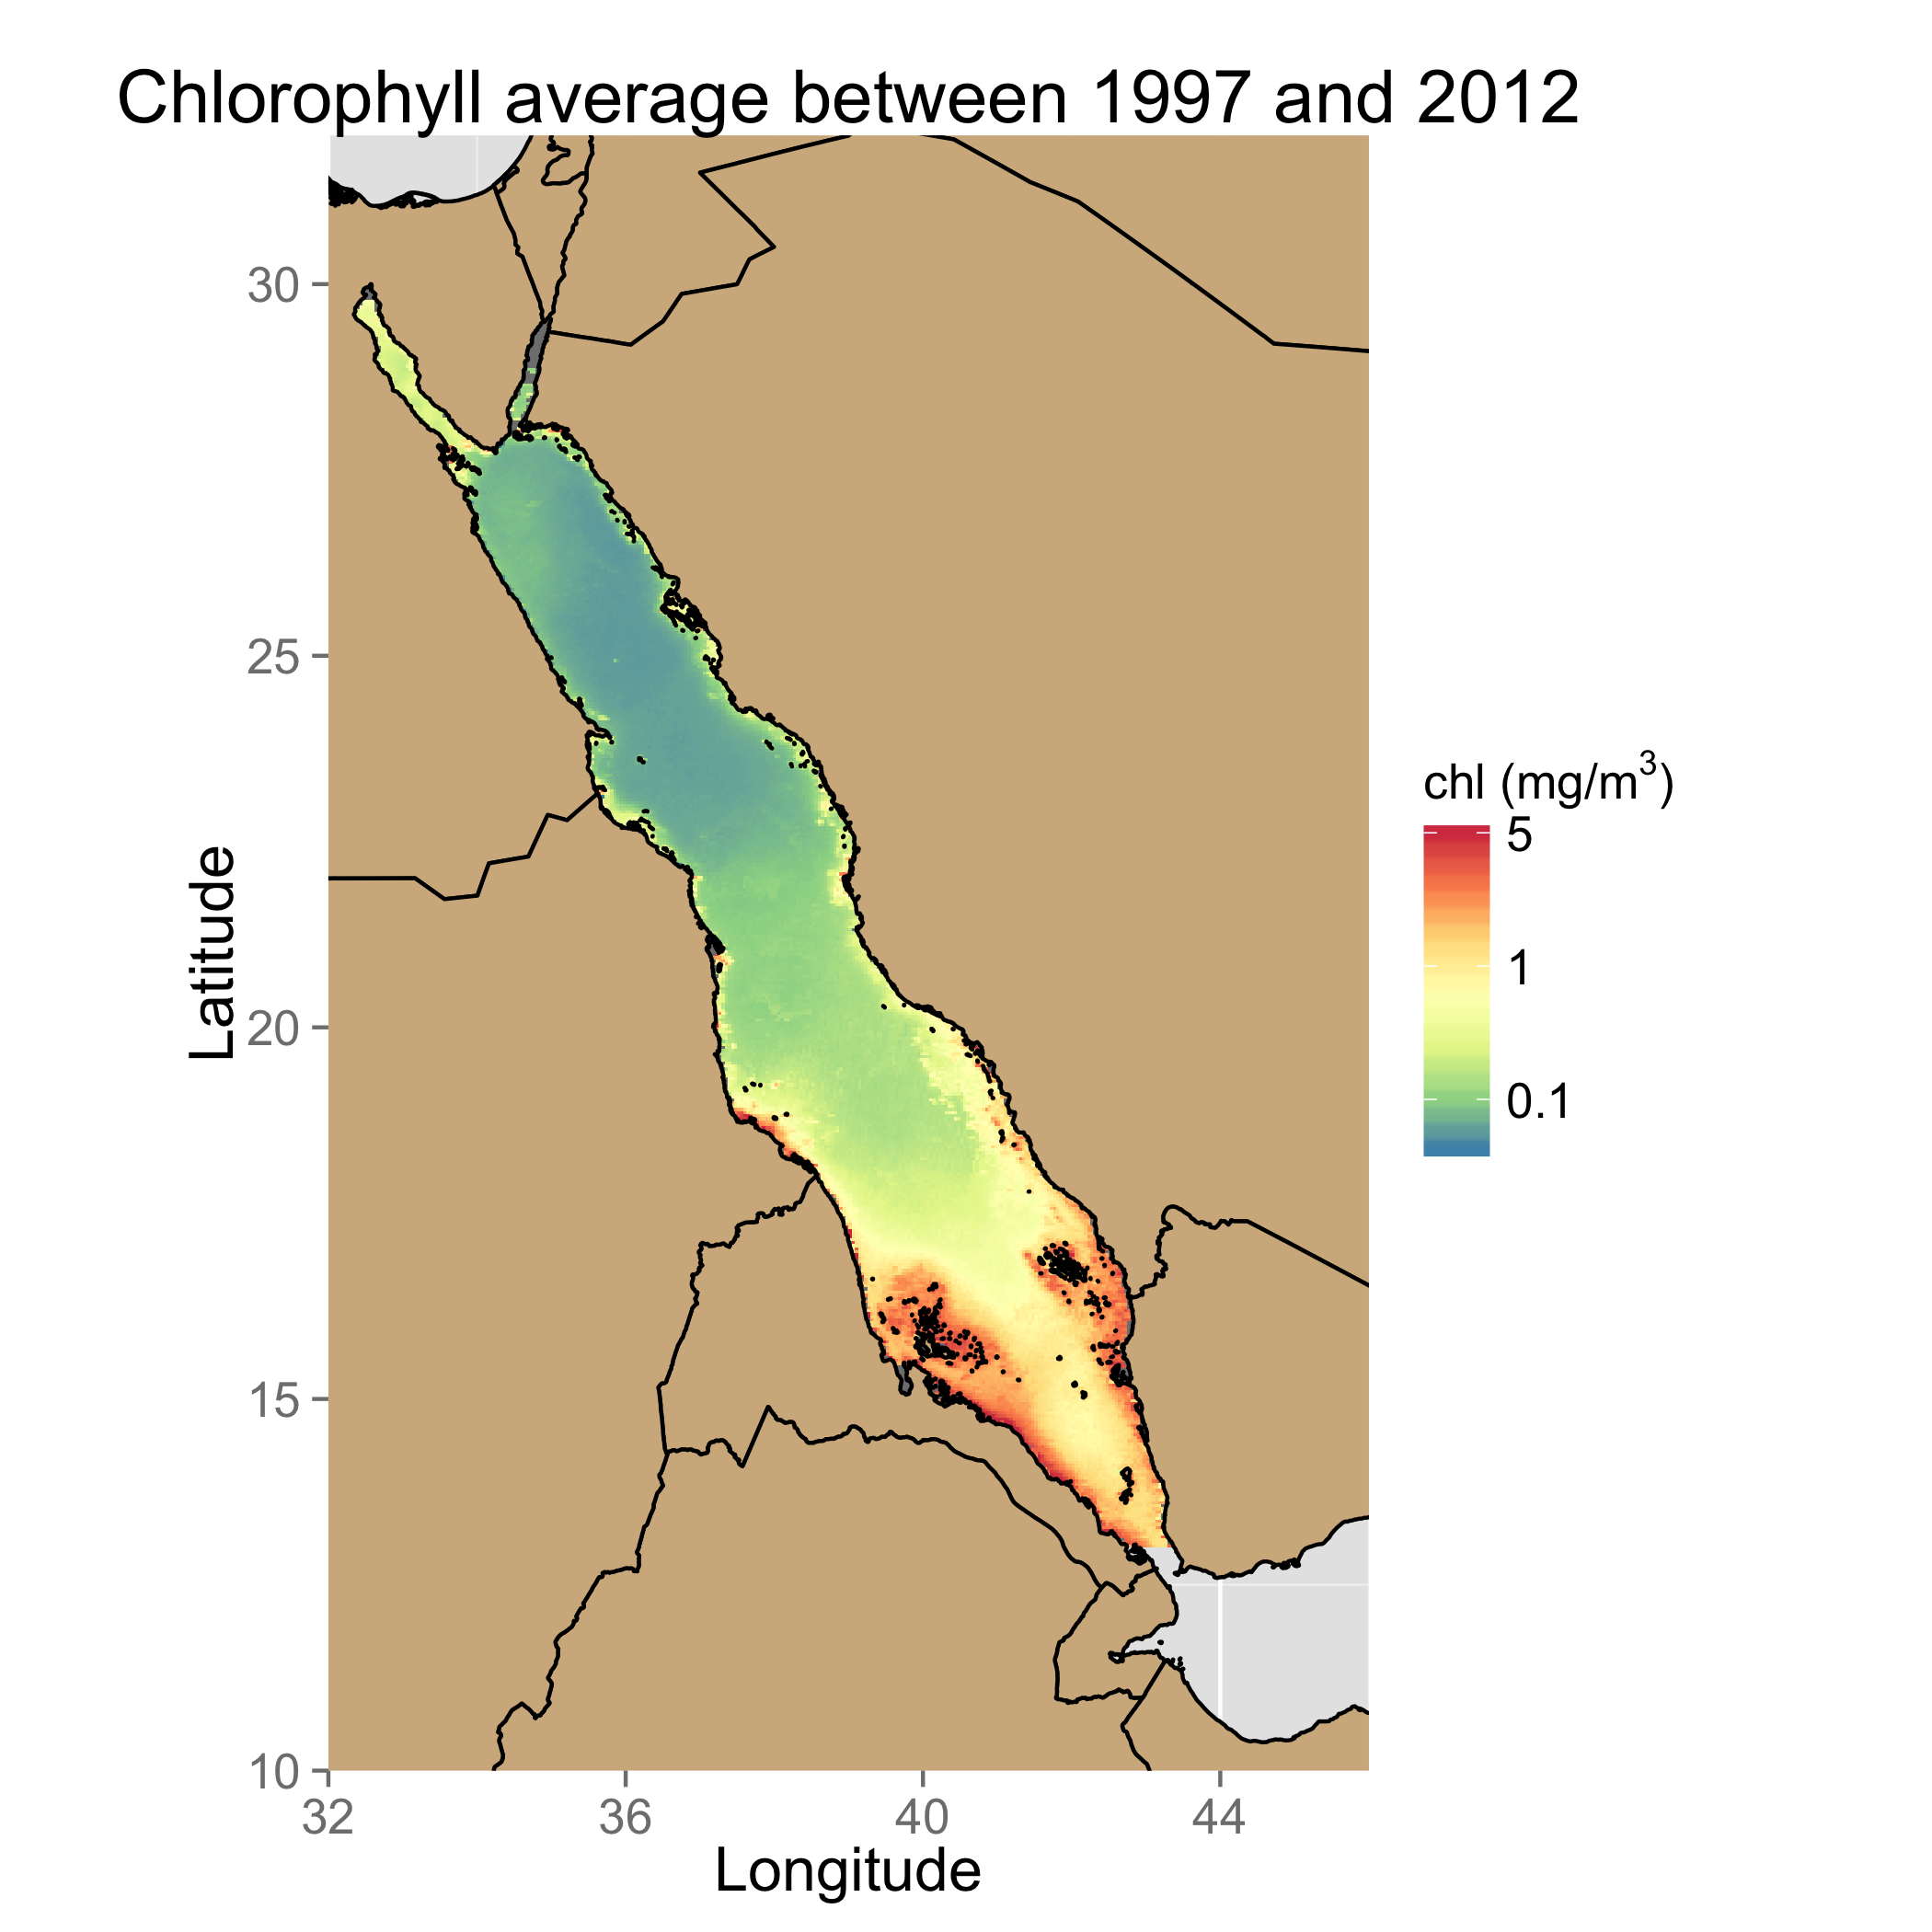
\includegraphics[scale=.15]{figures/chl_average.png}
    \caption{Average chlorophyll concentration from CCI data}
    \label{meanchl}
\end{figure}

The exchange of water with the nutrient-rich Gulf of Aden is a major driving
mechanism of the Red Sea productivity \citep{Triantafyllou2014}. It is believed
to be the most important source of nutrients. The maximum chlorophyll
concentration observed in the southern Red Sea during winter is attributed to
wind-driven water intrusion \citep{Raitsos2013, Yao2014}. In Summer, this
exchange of water is believed to be the major source of nutrients for the whole
Red Sea. The influence of the water intrusion weakens as the latitude
increases, explaining the low concentration in the northern half of the Red Sea
\citep{Raitsos2013}.

Deep convection also plays an important role in allowing nutrient-rich deep
water to mix with water of the euphotic zone. Vertical mixing is the most
vigorous in the northern extremity of the Red Sea during winter. This
explains its higher chlorophyll concentration compared to the north-central Red
Sea, a region of weak mixing \citep{Raitsos2013}. The northern Red Sea mixing
is believed to be mainly driven by wind \citep{Raitsos2013}.

The Red Sea circulation is strongly influenced by mesoscale eddies
\citep{Yao2014, Yao2014b, Zhan2014} that could impact primary production
\citep{Zhai2013}. In particular, the anti-cyclonic eddy in the central Red Sea
is believed to drive the June concentration peak and the summer productivity
of this region, by transporting nutrients and/or phytoplankton from the
adjacent coral reefs \citep{Raitsos2013}. In the northern Red Sea, a cold-core
eddy plays a role in enhancing the vertical mixing in this region
\citep{Raitsos2013}.

Aerial depositions of dust could also be an important input of nutrients for
the Red Sea, but it has been largely left unexplored \citep{Triantafyllou2014}.
\citet{Raitsos2013} noticed for example that sand storms in the Red Sea most
frequently happen in June and July, which coincides with the summer chlorophyll
peak. Finally, climate mode indices have been shown to be strongly correlated
with air-sea heat exchanges in the Red Sea \citep{Abualnaja2015}, and might
therefore influence its biology. This has been recently confirmed by
\citet{Raitsos2015}, who have shown that El Nino has a positive impact on the
chlorophyll concentration, by strenghtening the wind transporting nutrients
into the Red Sea from the Gulf of Aden.

\section{Remotely-Sensed Chlorophyll Data: Relevance and Challenges for the Red
Sea}

\subsection{Measuring Chlorophyll Concentration}

Chlorophyll is a molecule present in algae, phytoplankton and plants that is
critical for photosynthesis. It is a poor absorber of green light, and is
responsible for the coloration of plants \citep{Pal2014}. When phytoplankton
are present in high concentrations, the water usually takes a detectable green
coloration (it may also take a red or blue coloration depending on the type of
dominating phytoplankton) \citep{Robinson2010}. This offers an efficient way to
monitor the phytoplankton concentration from space.

In-situ measurement of chlorophyll concentration can be gathered through
scientific cruises, buoy stations or gliders (unmanned submarines). These
methods are expensive to deploy and therefore generally have limited temporal
and spatial coverage \citep{Robinson2010}. Political issues, as in the Red Sea,
as well as security issues, as in the Arabian Sea, set also barriers to in-situ
measurements.

Satellite measurements of chlorophyll provide excellent proxies for
phytoplankton concentrations with a good temporal and spatial coverage
\citep{Robinson2010}. The SeaWIFS, MODIS and MERIS missions have provided an
uninterrupted coverage of global ocean since 1997. High-resolution maps of
daily chlorophyll concentration are freely accessible to the scientific
community \citep{McClain2009}. Despite some limitations, such as missing data
due to cloud coverage and sunglint, or problematic values in coastal areas,
remotely-sensed chlorophyll concentrations are intensively used by the
scientific community. In regions, like in the Red Sea, where little in-situ
measurements are available, these constitute the most important data source
\citep{Raitsos2013, Brewin2013}.

\subsection{Limitation of Remotely-Sensed Chlorophyll Data in the Red Sea}

The quality of remotely-sensed chlorophyll data products such as MODIS and
SeaWiFS in the Red Sea is comparable with that of the rest of the world for
case I waters (open sea) \citep{Brewin2013}. However, the data contains a large
amount of missing values because of persistent clouds, sun-glint and sensor
saturation \citep{Racault}. This problem is particularly acute during the
summer in the southern Red Sea where the data coverage is almost null
\citep{Racault}, as shown in Figure \ref{misval_modis}.

Chlorophyll concentration estimation in optically complex case II waters is a
recurrent problem in this remotely-sensed data that particularly affects the
southern Red Sea.  In this region, the remotely sensed chlorophyll data could
be overestimated \citep{Raitsos2013}. However, all high values are not
necessarily wrong, as highly productive coral reefs are also present in this
region \citep{Raitsos2013}. These values have however not been validated yet,
because of the lack of in situ measurements \citep{Raitsos2013}.

\begin{figure}[h]
    \centering
    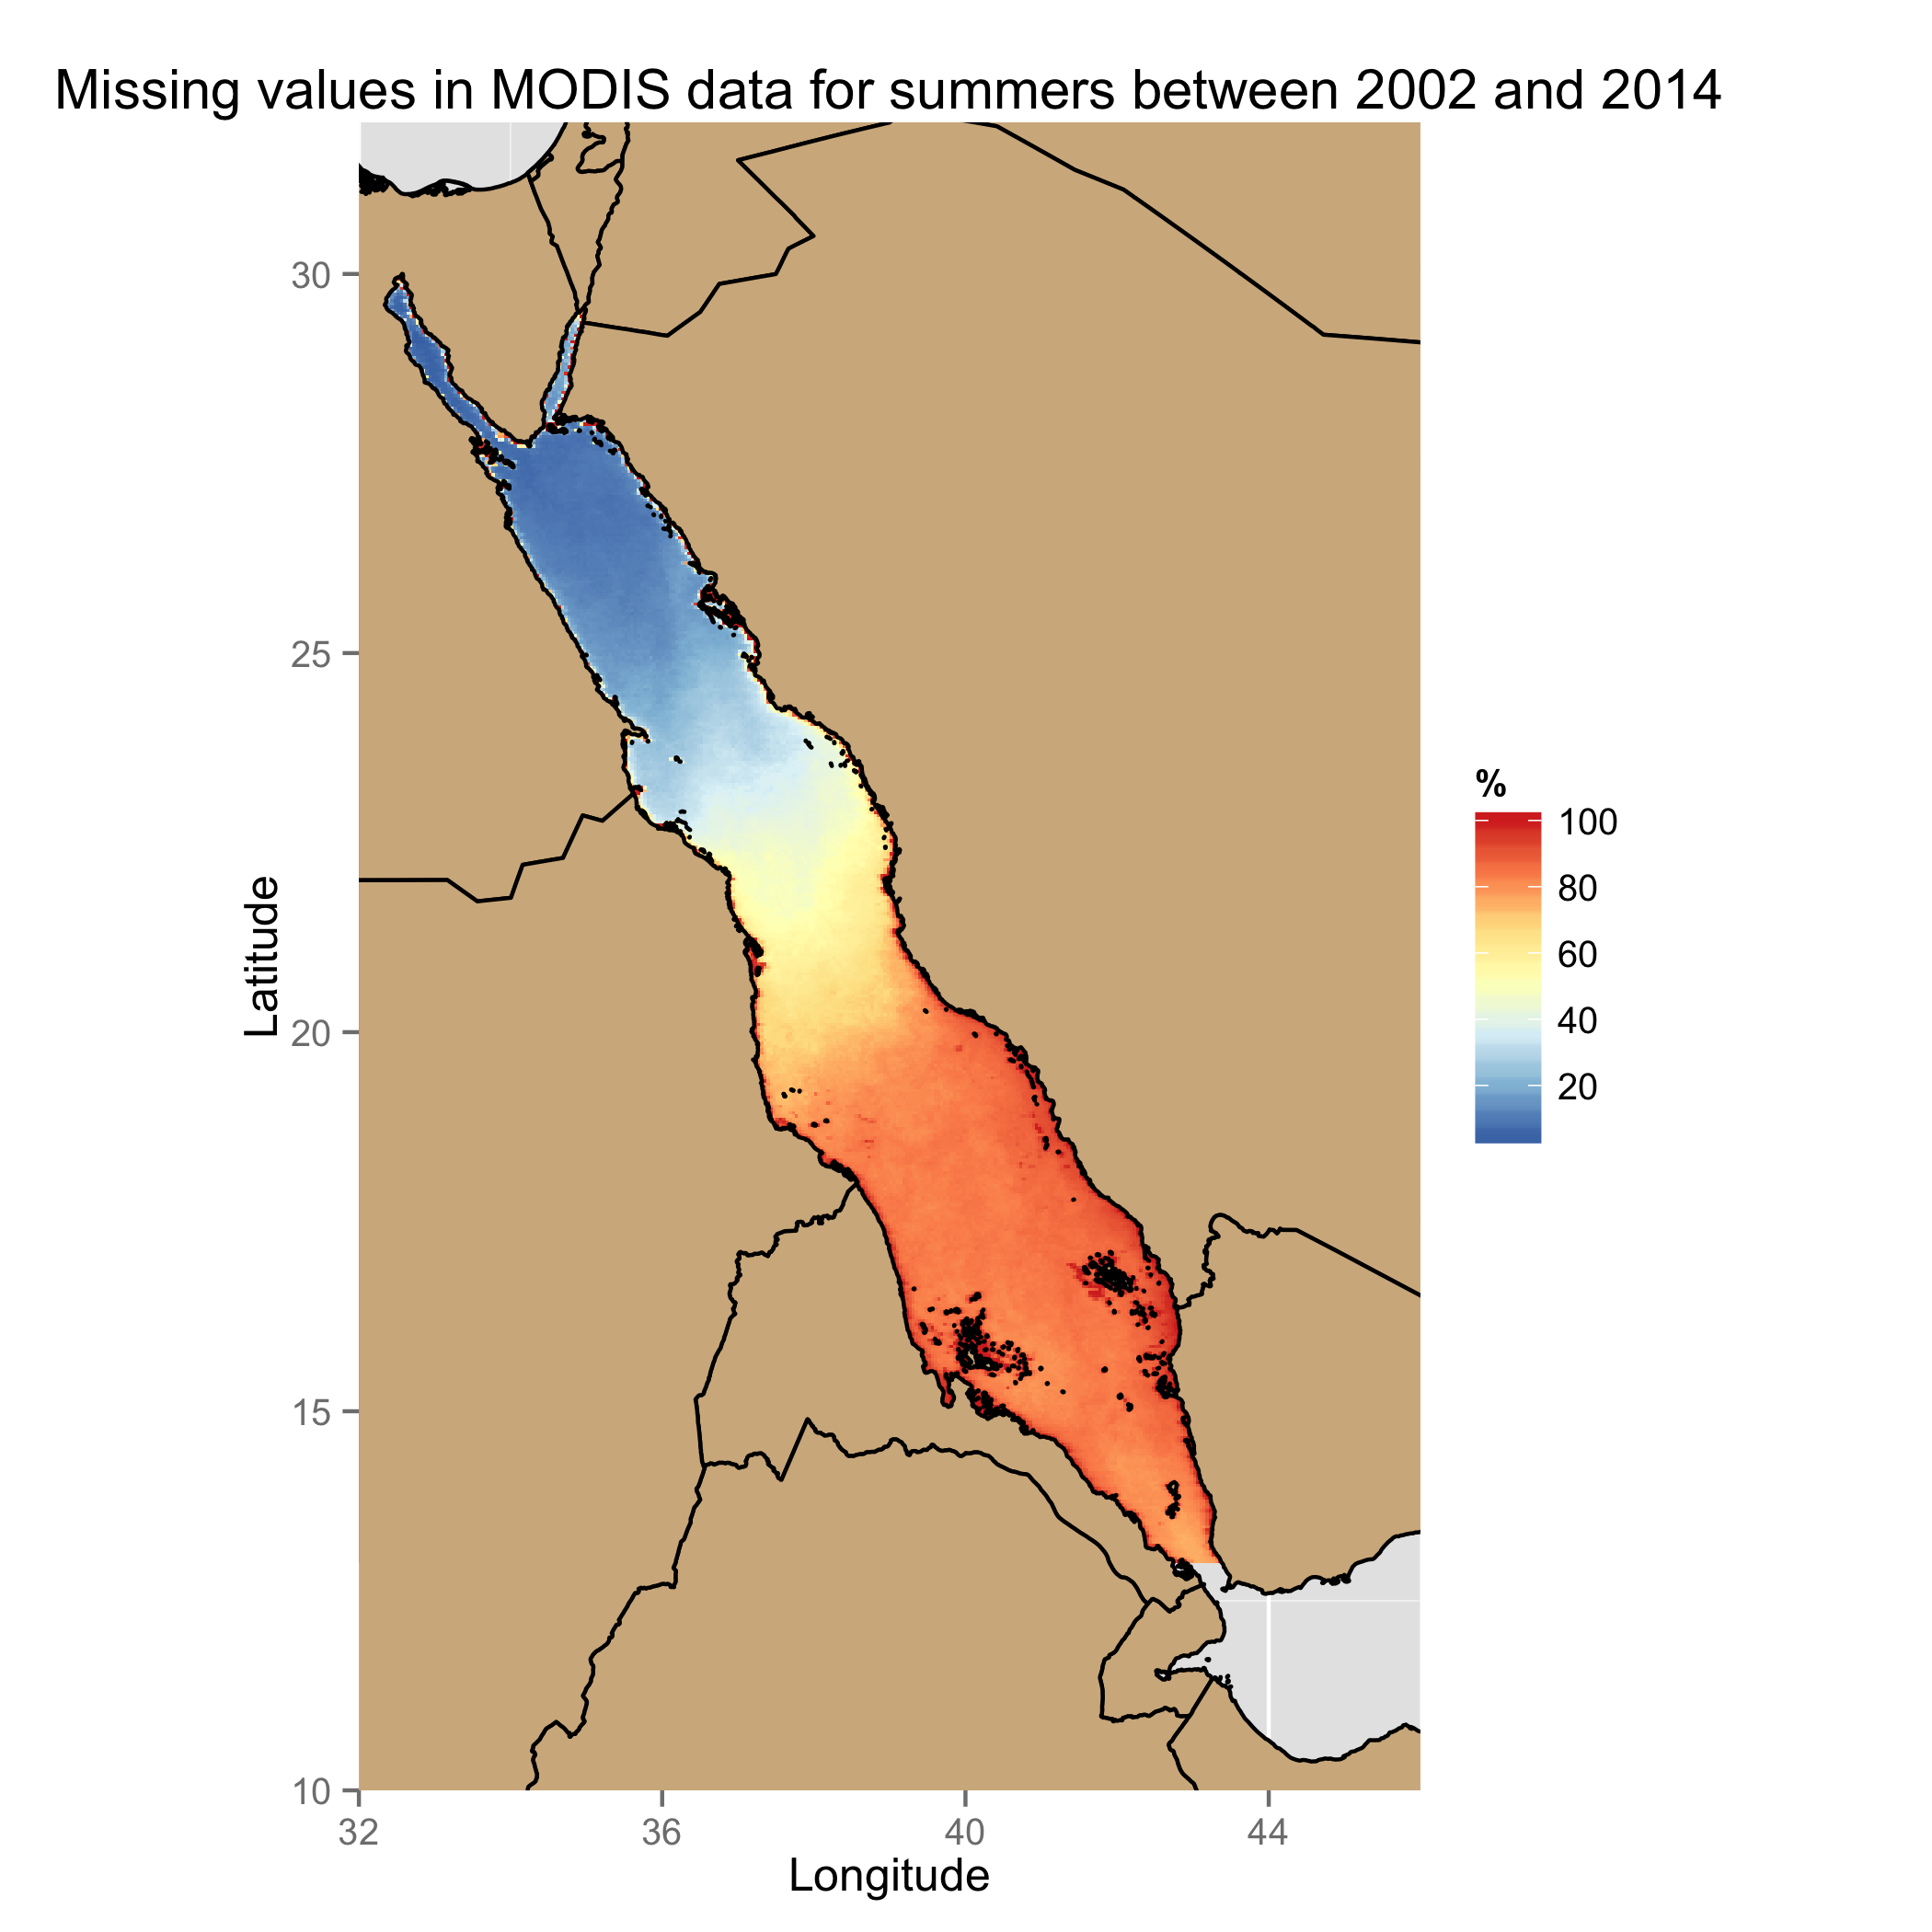
\includegraphics[scale=.15]{figures/modis_missing_values_summer.png}
    \caption{Percentage of missing values in the MODIS chlorophyll dataset}
    \label{misval_modis}
\end{figure}

One solution to missing and bad values is to apply a data filling algorithm, of
which one of the most popular algorithm is the Date INterpolating Empirical
Orthogonal Functions (DINEOF), which is an EOF based data filling approach
introduced by \citet{Beckers2003}. In \citet{Sicarjobs2011}, it has been
employed to fill chlorophyll data with 70\% of missing values.
\citet{Taylor2013} compared DINEOF with other EOF-based reconstruction
algorithms, suggesting that the former is a better method for data filling.
DINEOF has been further employed in several other chlorophyll studies
\citep{Miles2010, Waite2013}, and has also been used for multivariate
reconstruction of SST fields using chlorophyll data in \citet{Alvera2007}. 

The OC-CCI is a new chlorophyll data product that considerably increases the
Red Sea coverage. It is a merged product from the SeaWiFS, MODIS and MERIS data
missions.  Overall, it achieves a 75-80\% coverage in the entire Red Sea basin
against 50-65\% for a single sensor \citep{Racault}. During the summer, the
improvement in coverage is dramatic, as shown in Figure \ref{misval_cci}.
This is mostly
due to the use of the POLYMER algorithm \citep{Steinmetz2011} that allows to
exploit MERIS data collected during hazy conditions. This new dataset
has not been fully studied to revisit the assumptions made on the large-scale
Red Sea phytoplankton productivity.

\begin{figure}[h]
    \centering
    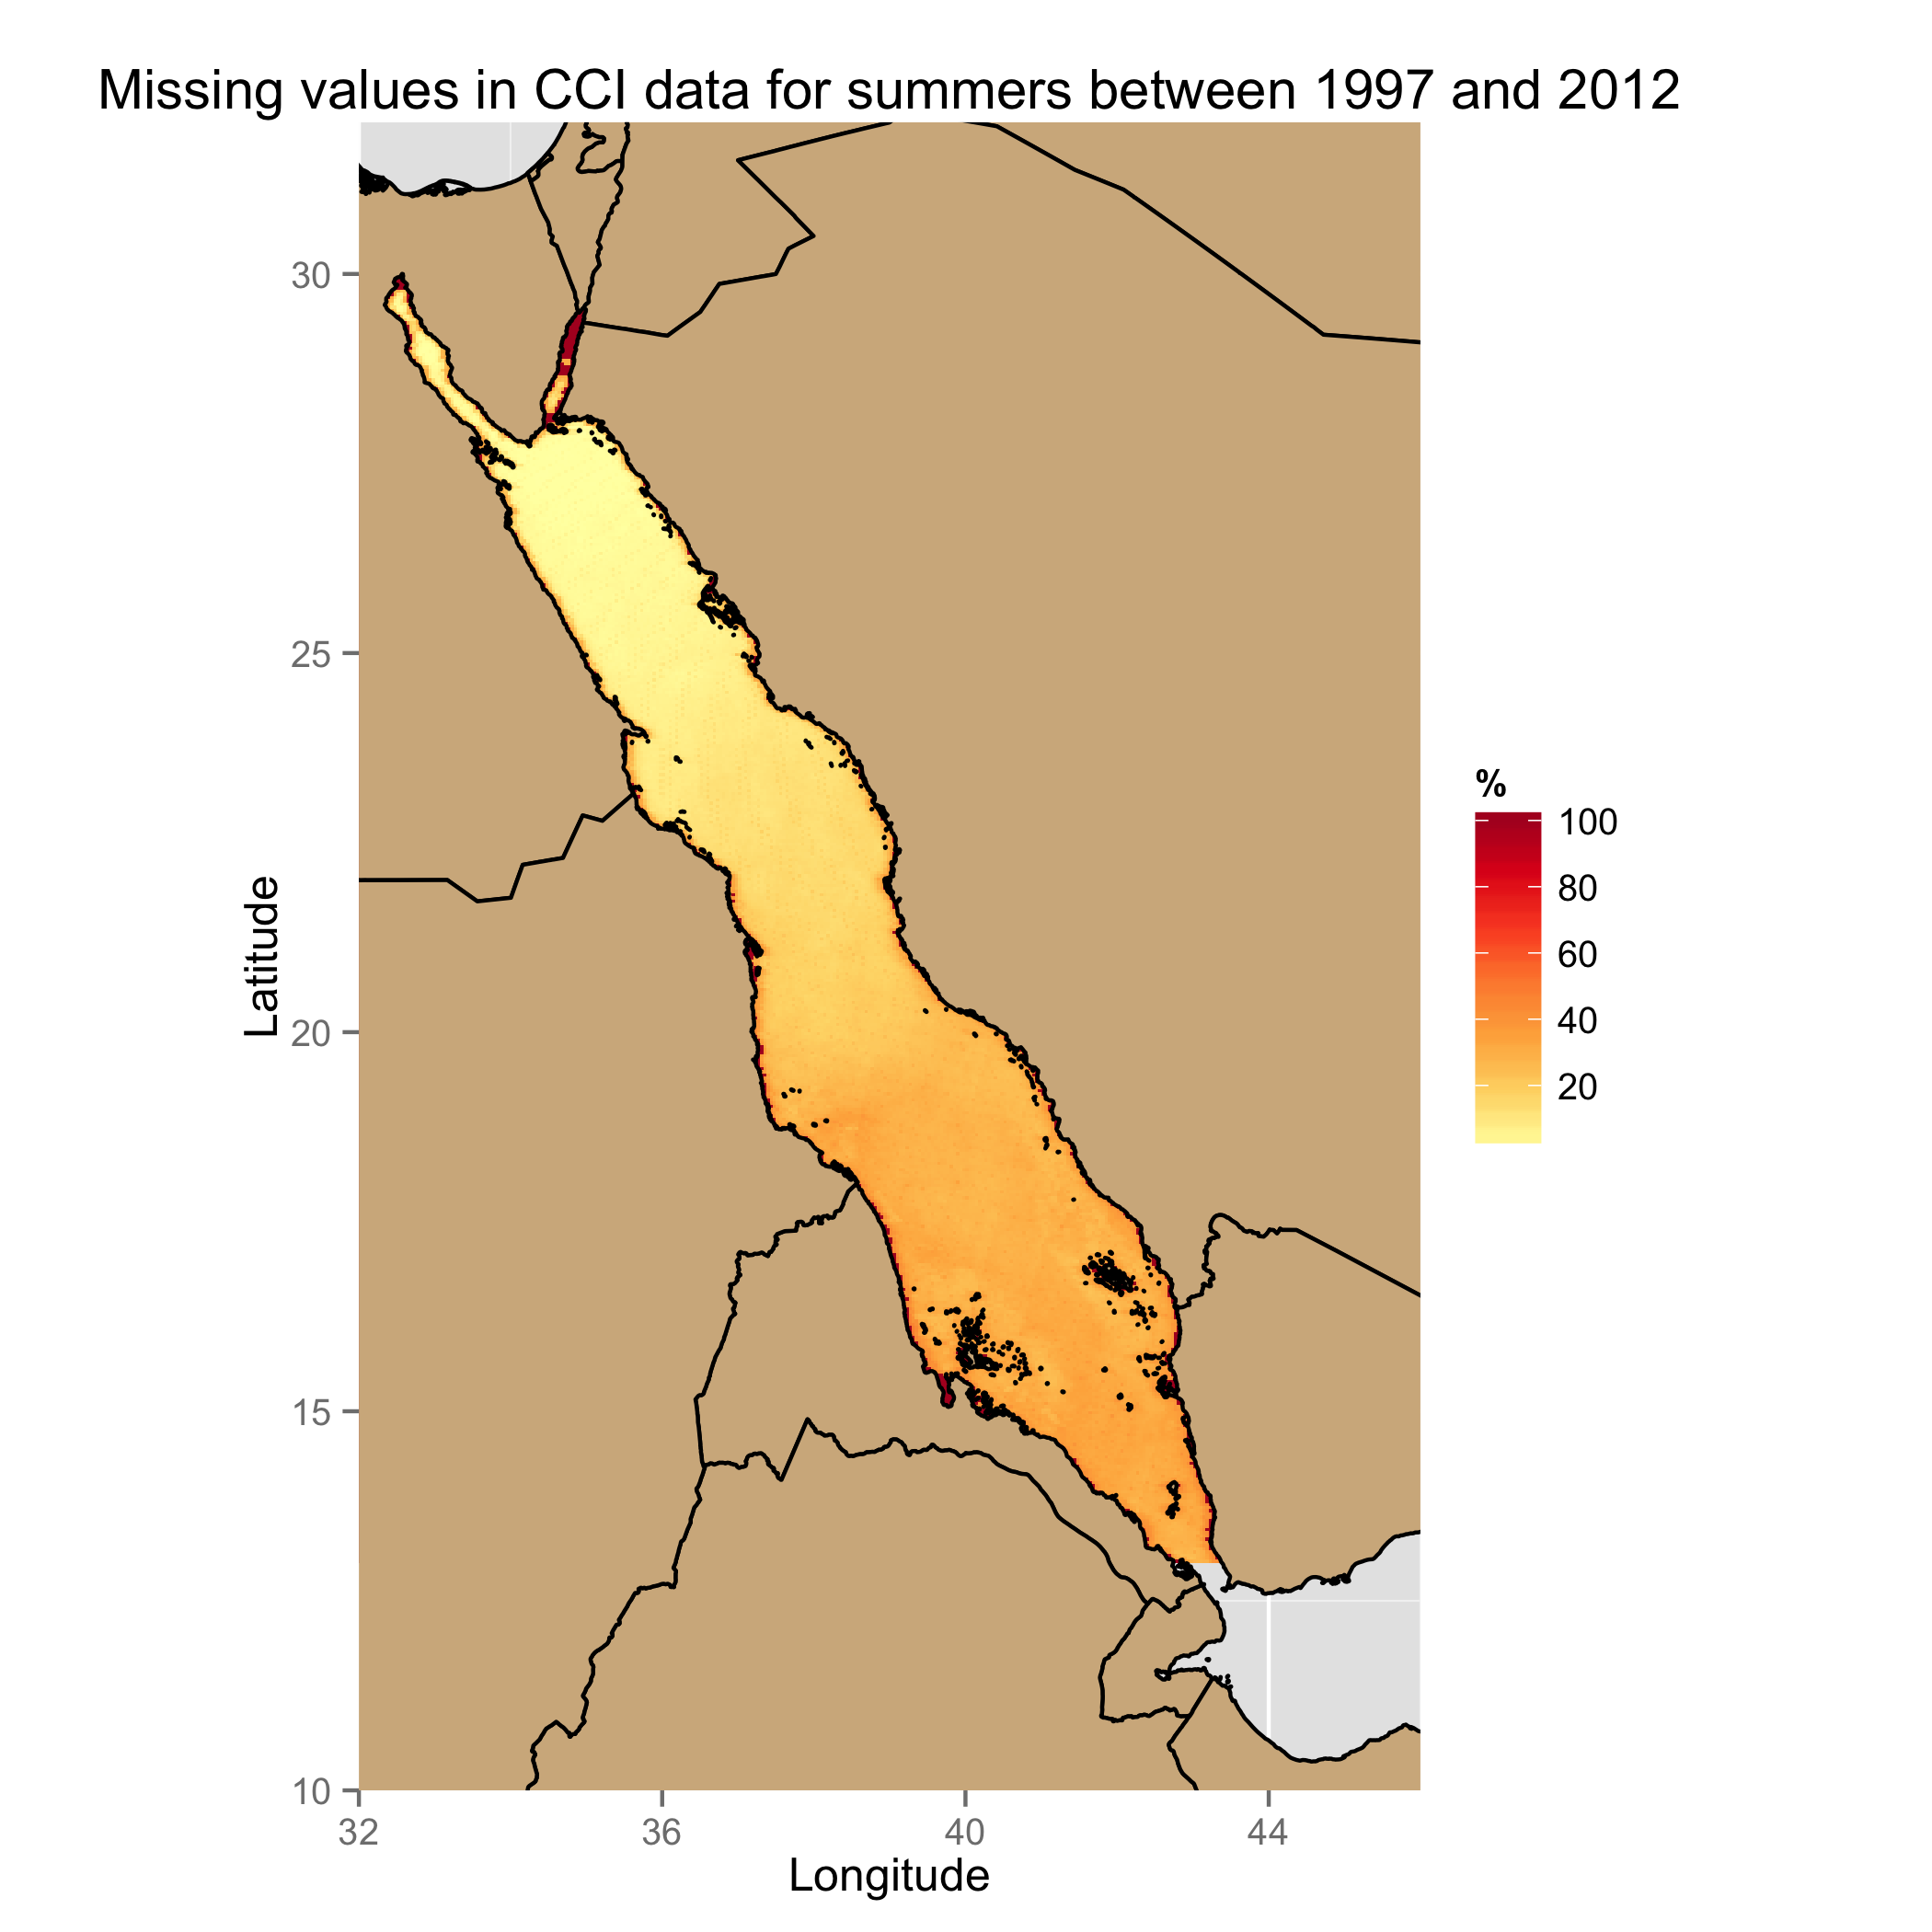
\includegraphics[scale=.15]{figures/cci_missing_values_summer.png}
    \caption{Percentage of missing values in the CCI chlorophyll dataset}
    \label{misval_cci}
\end{figure}

\section{Modeling and Forecasting Chlorophyll: Data and Dynamics Driven
Approaches, and Applications}

\subsection{Why Modeling Chlorophyll?}

Models could be useful to identify causes behind observed chlorophyll patterns.
Many hypotheses have been made about the drivers of chlorophyll concentration
in this regions, but some of them have not been yet investigated through
models. The role played by the exchange of water with the Gulf of Aden and
winter overturning in the northern Red Sea have been successfully modeled with
a 3D coupled physical-ecological model \citep{Yao2014, Yao2014b,
Triantafyllou2014}.  However, the interaction between the open sea and coral
reefs, and the role of atmospheric depositions have not been investigated yet.
Models, can also be helpful for understanding governing dynamics affecting the
chlorophyll concentration. In particular, the interaction between the
productivity level of the different regions of the Red Sea is yet to be
explored.

Model predictions of chlorophyll concentration also have practical applications
for fisheries. Furthermore, phytoplankton blooms can be harmful to humans and
marine life and are closely monitored in many regions of the world
\citep{Pettersson2013}. In the Red Sea, where tourism and aquaculture are
developing, it is likely to become a concern too. Phytoplankton is also
directly, and indirectly through zooplankton, the cause of microfouling that
affects desalination plants. In 2008-2009, a red tide forced the shutdown of
desalination plants along the Gulf of Oman and the Arabian Gulf
\citep{Richlen2010}.


\subsection{Deterministic Models}

\subsubsection{Ecological Models}

There is a rich literature on the modeling of marine ecosystems using
differential equations (see \citet{Fennel2004} for an introduction). In these
models the interactions of complex physical, chemical and biological processes
are modeled by differential equations that represent the flow of carbon,
nitrogen, phosphate and silicon. The biota is divided into trophic levels, and
can be further divided by feeding methods and size classes
\citep{Baretta1995, Triantafyllou2014}.

Ecological deterministic models vary widely in complexity depending on
the number of interactions represented.  They can be as
simple as the nutrient-phytoplankton-zooplankton (NPZ) model
\citep{Anderson2005} that only has three variables representing two trophic
levels and nitrate, or as complex as the European regional seas ecosystem model
(ERSEM) that has dozens of variables \citep{Baretta1995}. NPZ models are
extensively used because of their simplicity and capacity to model the the
large-scale features of marine ecosystems \citep{Anderson2005}.
ERSEM has recently been coupled to the MITgcm circulation
model used to simulate the Red Sea ecology \citep{Triantafyllou2014}. However
the complexity of these models makes them difficult to parametrize when not
enough data are available, which is usually the case in many marginal seas
\citep{Anderson2005}. Ecological models usually have large uncertainties due to
the imperfect modelization, the unknown initial conditions and the
uncertainties in the parametrization \citep{Edwards2015}.

\subsubsection{Data Assimilation}

Data assimilation is used to improve the simulations of ecological dynamical
models and enhance their forecasting capabilities by constraining their
predictions with available observations \cite{Edwards2015}. Such prediction
capabilities are deployed in operational expert systems, for example to study
the impact of human activities on the ecosystem of the Gulf of Pagasitikos
\citep{Korres2012}. The deployment of a similar forecasting system in the Red
Sea is currently under development \citep{Triantafyllou2014}. Hindcasting, the
estimation of unobserved variables, is another application of assimilation
systems. \citet{Ciavatta2011} showed that data assimilation of ocean color data
may improve the seasonal and annual hindcast of non-assimilated biogeochemical
properties in the shelf area of Western English Channel. Data assimilation can
also be used for reanalysis, to provide estimates of biogeochemical
distributions of the past \citep{Fontana2013}.

In the marine ecology modeling community, three assimilation schemes have been
widely used: the Ensemble Kalman filters (EnKF), the Singular Evolutive
Extended Kalman filter (SEEK), and its ensemble variant, the Singular Evolutive
Interpolated Kalman filter (SEIK). The stochastic EnKF, a Monte-Carlo
approximation of the Kalman Filter, has been used in \citet{Ciavatta2011,
Ciavatta2014}. This scheme may however suffer from sampling errors when the
ensemble size is smaller than the number of observations, as is usually the
case when assimilating remotely-sensed data \citep{Nerger2005, Altaf2014}.
SEEK is a reduced-rank variant of the Extended Kalman filter (EK). It was
introduced for efficient data assimilation into large scale ocean models.  It
is based  on the projection of the error covariance onto a low dimensional
space.  SEEK has a long history in data assimilation for marine ecology models
and is still extensively used in recent studies \citep{Fontana2013, Korres2012,
Butenschon2012}.  SEIK is an ensemble variant of the SEEK  and a deterministic
version of the EnKF that do not suffer from observations sampling errors, as it
updates the filter forecast exactly as in the Kalman filter. It therefore
requires a resampling step to generate a new analysis ensemble for the next
forecast step. SEIK has been used by \citet{Triantafyllou2013, Korres2012}.
\citet{Korres2012} shows that SEIK and SEEK are both comparably robust methods
for highly nonlinear systems. \citet{Hoteit2005} has shown that SEIK
outperforms SEEK when using a high-resolution nonlinear model.

Ecological models are challenging applications for state of the art data
assimilation schemes \citep{Edwards2015}. First, biogeochemical variables are
usually positive concentration, whereas Kalman filters expect Gaussian
variables, and log-transformation may fail to avoid this issue
\citep{Ciavatta2011}. In an attempt to mitigate this problem,
\citet{Fontana2013} introduced Gaussian anamorphosis transformations.
Second, ecological blooms are intermittent and highly nonlinear, conditions
that are challenging for Kalman filter-based assimilation schemes
\citep{Hoteit2005}. Third, SEIK, EnKF and SEEK project the
error covariance onto some subspace, resulting in an underestimation of the
estimation error. \citet{Butenschon2012} studied different ways to propagate
the error covariance in order to alleviate this issue. Finally, the model error
statistics are required by Kalman-derived filters, but are difficult to
estimate. \citet{Triantafyllou2013} proposed to use the $H_\infty$ method with
SEIK in order alleviate this requirement.

Particle filters represent a class of data assimilation schemes that, unlike
Kalman-based filters, do not require any linearity or Gaussianity assumption
\citep{Edwards2015}. As such, they might be more suitable for data assimilation
into ecosystem models. They have been studied in the case of 0D and 1D
ecological models \citep{Edwards2015}, but are still strongly limited by their
demanding computational requirements. Their application to 3D model is an
active field of research \citep{Edwards2015}.


\subsection{Data-Driven Approaches}

Compared to data assimilative ecological models, data-driven statistical models
are relatively simpler to develop. Such models are usually
relevant when the phenomenon
producing the data is dynamically complex to model, or simply poorly understood
\citep{Gareth2013}. Various data-driven models have been proposed
to predict chlorophyll
concentration, mostly in small regions with complex dynamics (see references
below). Some statistical models, such as linear regression, Gaussian additive
models, or tree regression have the advantage of being easy to interpret
\citep{Gareth2013}, and could be used to understand the dynamics driving the
chlorophyll concentration \citep{Raitsos2012}.

\subsubsection{Statistical Models}

Statistical and machine learning models have been recently used for estimation and
classification problems related to phytoplankton concentrations. One
application is the detection of harmful algal bloom from spatio-temporal
satellite dataset, that has been addressed by \citet{Gokaraju2011} in the Gulf
of Mexico using support vector machines. Another application is the estimation
of chlorophyll concentration in case II coastal water using satellite radiance
data. This problem has been considered by \citet{Kim2014} on the west coast of
South Korea, and by \citet{Camps-Valls2006} using a global dataset of in situ
measurements.  The former used the support vector regression algorithm, while
the latter used the random forest algorithm.

Machine learning algorithms, in particular Artificial Neural Networks,
are also very popular for forecasting regional chlorophyll concentration in regions
with very complex dynamics, where deterministic ecological models usually
perform poorly. Neural networks are also commonly used for forecasting
chlorophyll concentration in fresh as well as in coastal water systems. In
\citet{Jeong2006}, temporal recurrent recursive neural networks have been used
and found superior to traditional time-series models for daily forecasts of
chlorophyll concentration.  \citet{Wang2013} also used recurrent neural
networks for forecasting daily chlorophyll in Lake Taihu, China.
\citet{Mulia2013} combined Neural Network and genetic algorithm for nowcasting
and forecasting of the chlorophyll concentration up to 14 days ahead, in the
tidal dominated coast of Singapore.  Finally, \citet{Lee2003} used neural
networks for the forecasting of algal bloom with one or two weeks lags in the
coastal waters of Hong-Kong.

\subsubsection{Geostatistics}

Phenomena such as propagation and diffusion play a key role in the chlorophyll
spatial concentration, but are difficult to represent without spatial modeling.
There is also a difference in the chlorophyll patterns of different regions of
the Red Sea, in particular between the nutrient rich southern Red Sea and the
oligotrophic northern Red Sea, and between the open ocean and the coastal
waters \citep{Raitsos2013}.  One should also expect the different regions of
the Red Sea to interact.

In contrast to the statistical models presented above, in geostatistical
models, the spatial dimension is modeled explicitely by representing the data
as a spatial stochastic process \citep{Gneiting2007}. In classical
geostatistics, spatial data is modeled as the realization of a two- (or three-)
dimensional Gaussian process \citep{Gneiting2007}.  Geostatistics can be easily
extended to spatio-temporal datasets \citep{Gneiting2007}. Many ways for
constructing space-time covariance functions for these models have been
recently proposed \citep{Gneiting2002, Cressie1999, Stein2005}.

The theory of space-time geostatistics is closely related to that of spatial
statistics. In fact, the time dimension becomes an additional dimension. However,
the relationship between these two dimensions is derived from a dynamical process,
that must be taken into account in the definition of the covariance function
\citep{Gneiting2010}. Some space-time covariance models can actually be derived
from a physical formulation, such as the frozen fields \citep{Gneiting2010}, or
stochastic differential equations \citep{Brown2000, North2011}.

Physically-derived space-time covariance functions are not commonly used, and
the usual approach is to construct them from spatial and temporal covariance
functions \citep{Gneiting2010}. One of the most simple types are separable
covariance functions, that are the products of a spatial covariance function
and temporal covariance function. These are computationally efficient, but are
not suitable to represent space-time interactions \citep{Cressie1999,
Stein2005}, making them of limited use for modeling physical systems. The
Cressie, Huang spectral characterization theorem of space-time covariance
functions has opened the door to wider ways of constructing them. For example,
\citet{Gneiting2002} presented a simple criterion that allows their
construction from a very large class of models. 

Space-time geostatistical models have been used in a variety of applications.
\citet{Hohn1993} used it for forecasting the outbreaks of an invasive specie.
These methods have also been used in meteorology to model temperature fields
\citep{Handcock1994, North2011} or wind \citep{Cressie1999, Gneiting2002}, and
in environmental studies for ground-level ozone concentration. However,
they have not been applied to chlorophyll data.

\section{Thesis Objectives}

There is a crucial need for improving the modeling of large-scale features of
marine ecosystems. The ocean physical, chemical and ecological processes are
complex and poorly understood. Even though ocean color remote-sensing data has
revolutionized our understanding of marine ecology, it only gives information
about the phytoplankton at the sea surface. Our knowledge is even more limited
in the Red Sea, due to the paucity of in situ data.

The goal of this thesis is to develop novel models for efficient forecasting of
chlorophyll concentration in the Red Sea. Various methods will be developed and
tested following data and a dynamical-driven approaches. In particular, we will
develop efficient approaches to model the Red Sea chlorophyll, explore the
possibility of improving the state of the art data assimilative ecosystem
modeling, and introduce the use of geostatistics to the field of marine
ecology. The merits of both approaches will be compared for the first time in
the same region, and under the sames conditions. We will also propose ways to
efficiently combine both approaches methods for best forecasting of chlorophyll
concentration.

Currently, both deterministic and statistical approaches have been used to
predict chlorophyll. However, these approaches have never been compared, nor
combined in the same problem. A thorough comparison is very much needed. It
would provide modelers with a comprehensive foundation for developing their
modeling strategy. Combining them may further improve the forecasting skills.

This thesis will also help increase our understanding of the Red Sea ecology.
In particular, it will identify possibles drivers for the chlorophyll
seasonality and interannual variability. We will also identify and characterize
the different Red Sea eco-regions. This work has practical applications for the
region. In particular, better forecasting phytoplankton blooms may be extremely
important for the operations of desalination plants and aquaculture.


\chapter{Research Plan}

\emph{Write some introductory text here}

\section{Task 1: Dataset building and Exploration}

\noindent
\emph{Duration: 2 months (by December 2014)}

\noindent
\emph{Submission: Journal of Marine Systems}

\noindent
\emph{Collaborator: Dionysios Raitsos}

\subsection{Motivation}

A preliminary task to data modeling, is the gathering, cleaning and exploration of the data. Given the complexity and the size (40 GB) of the data, this is not an easy task. This first data analysis, will reveal if enough data has been gathered to make meaningful forecast, and what accuracy we can expect from the models. This step will also provide information that will help in designing statistical models: most significant variables, differences between regions, relevant data transformation, etc. Finally, this step will identify patterns in the data that will be useful to qualitatively evaluate predictive models.

\subsection{Open Questions}

\begin{itemize}
\item Can we efficiently identify outliers in the chlorophyll values?
\item Is there a way to efficiently fill the missing values in the chlorophyll dataset?
\item Can the data help understanding the mechanisms behind extreme blooms in the Red Sea?
\item Can the hypothesizes about the dynamics behind the chlorophyll seasonal cycle be confirmed by the data?
\item Are there more blooms in the past years?
\end{itemize}

\subsection{Method and Work Done}

\begin{enumerate}
\item Identify data sources and load the data…………………………………………………60%
\item Clean the data and fill missing values (DINEOF)......................................................50%
\item Align and format the data in order to have a unique dataset…………………………...0%
\item Explore the dataset………………………………………………………………………..20%
\begin{itemize}
\item Study the correlation between chlorophyll and other variables (Linear Regression, GAM, data transformations)
\item Select variables (Lasso, single variable regression, multistep regression)
\item Study the regional aggregation (ACF)
\item Explore spatiotemporal correlations (hovmoller plots, PCA, variograms)
\item Estimate the Bayes factor/ % of variance explained (k-nearest neighbors)
\end{itemize}
\end{enumerate}

\subsection{Expected Outcomes}

\begin{itemize}
\item A cleaned dataset that can be used in the following tasks
\item A comprehensive exploration of the available data for chlorophyll study in the Red Sea
\item A preliminary variable selection
\item A clear picture of the major spatio-temporal patterns in the data
\item A critical evaluation of the current hypothesis about the chlorophyll dynamics in the Red Sea
\end{itemize}

\subsection{Work Accomplished and Prelimnary results}

\section{Chapter 2: Forecasting Chlorophyll Concentration in Regional Aggregates}

\noindent
\emph{Duration: 2 months (by February 2015)}

\noindent
\emph{Submission: Progress in Oceanography}

\noindent
\emph{Collaborator: Dionysios Raitsos}

\paragraph{Motivation}

Chlorophyll data is very complex. It is therefore useful to first simplify it by aggregating it spatially. The space-time dynamics of the chlorophyll data reflects the highly nonlinear dynamics of the underlying physical, chemical and biological phenomenons. As shown by the north-south gradient and the seasonal behavior, the resulting space-time process is nonstationary in time and in space. The high-dimensionality in space can be reduced by considering a regional aggregation of the results. This would allow us to focus on the global scale phenomenons: such as the interactions between neighboring regions, the time-scale of large events and the difference in the physical variables affecting the chlorophyll concentration in each region. In the following tasks, these simple predictive models will also be a reference for evaluating more complex ones. 

\paragraph{Open Questions}

\begin{itemize}
\item Is the biological aggregation of the Red Sea proposed by (Raitsos 2013) statistically meaningful?
\item Can clustering methods be used to identify marine ecological zones based on chlorophyll data?
\item Can a simple forecasting model allow us to understand the causes of chlorophyll blooms?
\item Can the current hypothesizes about the seasonal chlorophyll dynamics be validated?
\end{itemize}

\paragraph{Method}

\begin{enumerate}
\item Define datasets (training and test datasets, cross-validation).....................................0%
\item Variable selection (Lasso, L1 regression, single-variable linear regression)...............0%
\item Define regional aggregations (unsupervised learning, Hierarchical clustering, K-means)...................................................................................................................50%
\item Forecasts chlorophyll concentration (linear regression, GAM models, diagnostic, k-nearest neighbors)....................................................................................................0%
\item Predicting future extreme blooms (nearest-neighbours, logistic regression, decision trees)...........................................................................................................................0%
\end{enumerate}

\paragraph{Expected Outcomes}

\begin{itemize}
\item A regional division of the Red Sea that has been quantitatively evaluated.
\item A critic of current hypothesis about the chlorophyll dynamics in the Red Sea.
\item A lower bound on the performance of a more sophisticated model.
\item An assessment of the limitation of aggregate methods for Chlorophyll data.
\item An understanding on how the treatment of spatial correlations can improve the results.
\end{itemize}

\paragraph{Work Accomplished and Prelimnary results}

\section{Chapter 3: Global geostatistical model for forecasting}

\noindent
\emph{Duration: 1 month (by March 2015)}

\noindent
\emph{Submission: Spatial Statistics}

\paragraph{Motivation}

Geostatistical methods can be used to construct dynamical models for forecasting the chlorophyll concentrations that we can compare to deterministic models. Geostatistics is a robust method to model spatio-temporal data. Recently there has been a lot of research on expanding it to model spatio-temporal data. With Kriging, these models a are powerful ways to do spatio-temporal prediction. As a particular case of Kriging, by predicting the spatial future field given the observation of the present field, we can derive a linear dynamical model. This linear model can be employed in a filtering setting like the Kalman filter. This is a desirable setup, as it is similar to the way deterministic models are employed to do forecasts given past observations. 

\paragraph{Open Questions}

\begin{itemize}
\item Can a global geostatistical model fit chlorophyll data?
\item How non stationary is the data in time and space?
\item What spatiotemporal covariance functions best fit the chlorophyll data?
\item Can geostatistical methods be employed in a filtering setup?
\end{itemize}

\paragraph{Method}

This task has already been started and had been the object of a submission for publication. The remaining work includes:
Use the new dataset and the new covariates
Compare the results to the ones of with the regional aggregates
Expected Outcomes
A methodology to employ a geostatistical model in a filtering problem.
A characterization of the space-time non stationarity of the data, and the interaction of the temporal and spatial dimensions.
An understanding of how spatial aggregation and geostatistical models can be used in the same model. 

\paragraph{Work Accomplished and Preliminary Results}



\section{Task 4: Local geostatistical model for forecasting}

\noindent
\emph{Duration: 3 months (by June 2015)}

\noindent
\emph{Submission: Journal of the American Statistical Association (Case Study)}

\noindent
\emph{Collaborator: Raphael Huser}

\subsection{Motivation}

This part will bring together the results of the two preceding tasks to develop a predictive model that takes into account the large-scale dynamics and the regional spatio-temporal dynamics. In task 2, a predictive model is built, that represents the large scales behaviour of the Red Sea, but the spatial dimension inside each region is not addressed. We expect local features to play a role, such as the proximity to the coast, the bathymetry, proximity to other regions or major cities, etc. In task 3, we developed a methodology to use a geostatistical model in a dynamic fashion to do pixel-scale forecast. In this task, each regions will be modeled separately by a local geostatistical model that can do local prediction. These models will have access to aggregate covariates from neighboring regions in represent the global scale behaviours. 

\subsection{Open Questions}

\begin{itemize}
\item What are the most adapted space-time covariance models for chlorophyll data?
\item How to use global covariates in a geostatistical model?
\item What are the differences in the fine-scale dynamics of chlorophyll in each region?
\item Can the fine scale behaviour of phytoplankton be predicted accurately?
\item What are the spatial features that are important for the chlorophyll dynamics?
\end{itemize}

\subsection{Method}

\begin{itemize}
\item Extract local dataset from previous tasks
\item Design the training and test datasets, and the cross-validation method
\item Design and evaluate the mean function given the past covariates
\item Fit the local geostatistical model to the residuals.
\item Evaluate the model predictions and compare the results with task 2 and 3.
\end{itemize}

\subsection{Expected Outcomes}

\begin{itemize}
\item A methodology to aggregate local geostatistical models
\item An improvements in the prediction skills over the models of task 2 and 3.
\item An understanding of the differences between each regions.
\item A critical evaluation of the space-time covariance models for fitting chlorophyll data.
\item A better characterization of the regional chlorophyll dynamics.
\end{itemize}

\section{Chapter 5: Assimilation of 1D ecological models and comparison to statistical models}

\noindent
\emph{Duration: 3 months (by September 2015)}

\noindent
\emph{Submission: Journal of Geophysical Research}

\noindent
\emph{Collaborator: George Triantafyllou / Boujeema}

\paragraph{Motivation}

The three previous tasks focus on constructing increasingly sophisticated predictive models for the chlorophyll concentration in the Red Sea. In this part these models will be compared to a 1D ecological model (ERSEM). This model is well detailed and very complex. The goal of this part will be to identify the merits of each modeling approach, and propose ways in which they can complement each other. To allow for comparison, the model will be run in each of the regions found in task 2. Available data will also be assimilated to the model through a smoothing assimilation scheme that will use an expectation-maximization algorithm for parameters estimation. 

\paragraph{Open Questions}

\begin{itemize}
\item Are statistical methods competitive for forecasting chlorophyll concentrations?
\item How can statistical and deterministic models complements each other?
\item Can statistical method forecast interesting dynamical features?
\item Are there significant regional differences in the relative performances of both approaches?
\item How to estimate the parameters of ecological models? 
\end{itemize}

\paragraph{Method}

\begin{enumerate}
\item Define the metrics for comparison
\item Calibrate the ERSEM model on each of the regions
\item Define an assimilation scheme and the data for the ERSEM model
\item Implement the assimilation scheme
\item Run the simulation and aggregate the results
\item Do the comparisons with the statistical models
\end{enumerate}

\paragraph{Expected Outcomes}

\begin{itemize}
\item A complete set of measures of the prediction skills of each approach.
\item A method to estimate assimilation and model parameters in an assimilated ecological model.
\item A set of case studies of the behaviours of each method for forecasting interesting events.
\item An understanding of the limitations of geostatistical models to predict nonlinear dynamics. 
\item Propositions on how the two approaches can complement each other.
\end{itemize}

\paragraph{Work Accomplished and Preliminary Results}


\section{Task 6: Improving an Ecological Model Data Assimilation Scheme through Statistical Predictive Models}

\noindent
\emph{Duration: 3 months (by September 2015)}

\noindent
\emph{Submission: Journal of Geophysical Research}

\noindent
\emph{Collaborator: George Triantafyllou / Boujeema}

\section{Motivation}

In the previous task, we compared the forecasts of the ecological ERSEM model to that of the statistical models we developed from tasks 2 to 4. In this task we will study how these two approaches can be complementary. Specifically, we will study the use of statistical forecasts model to improve the forecasts of the ERSEM ecological model. The forecasts of the statistical models will be treated as observations, that can be assimilated by the filtering scheme used with the ERSEM model, and will give an improved forecast. When real observations will be available, they will be assimilated sequentially. This, method will allow the different ERSEM models on each cluster to communicate indirectly their states to one another. 

\subsection{Open Questions}

\begin{itemize}
\item Can statistical predictive models be used to communicate information between deterministic model?
\item Would the access to information about other regions improve the model forecasts?
\item What are the global patterns of ecological dynamics in the Red Sea?
\end{itemize}

\subsection{Method}

\begin{enumerate}
\item Define new assimilation scheme
\item Define metrics to measure model improvement
\item Prepare training and test datasets
\item Train statistical model
\item Run simulation with assimilation of statistical observation
\item Compare with results of task 5
\end{enumerate}

\subsection{Expected Outcomes}

\begin{itemize}
\item An improvement in the prediction skills of the deterministic approach
\item A methodology to couple deterministic ecological models through statistical models
\item Insights on the global ecological dynamics of the Red Sea
\end{itemize}


\chapter{Summary of Progress}

\section{Data Preparation}

All of the datasets necessary for the analysis has been gathered. Almost all of
it has been downloaded from public sources on the Internet, using Shell and R
scripts.  The wind dataset has been provided by Yesubabu Viswanadhapalli, and
is the result of the assimilation of QuickScat satellite and in situ data to
the Weather Research and Forecasting (WRF) regional Red Sea model. There are
additional datasets that will be useful for the analysis, but they are mainly
climate mode time-series like IMI and EAWR, that are easy to download. The
downloaded data is listed in table \ref{tab:data}.

So far, the MODIS and CCI data have been cropped over the region of interest,
cleaned and exported to the format TIFF, which can be read easily by most
software, R in particular. Each dataset has then been aggregated in a single
file in the native R raster format. Applying this processing to the remaining
raster data should be straightforward. Then, the data will need to be aligned
and aggregated on the same temporal and spatial resolution, before aggregating
it in table format.

\afterpage{

%\clearpage% Flush earlier floats (otherwise order might not be correct)

\thispagestyle{empty}% empty page style (?)

\begin{landscape}% Landscape page
\begin{table}
\centering % Center table

\begin{tabular}{l c c r} 

\toprule 

Variable       &Description             & Mission/Source    & Unit       \\

\midrule 

CHL                     & Chlorophyll             & CCI               & mg/m${}^3$ \\ SST            &
Sea Surface Temperature & MODIS             & Celsius    \\ 

AOD            &Aerosol Optical Depth   & MODIS             & N/A        \\ 
CDOM           &  Colored Dissolved       & MODIS             & N/A        \\ 
& Organic Matter
&                   &            \\ NAO            & North Atlantic          &
NOAA              & N/A        \\ & Oscillation Index       &
&            \\ PAR            & Photosynthetically      & MODIS             &
Einstein / m${}^2$ . Day                                                \\ &
Available Radiations    &                   &            \\ POC            &
Particulate Organic     & MODIS             & mg/m${}^3$ \\ & Carbon
&                   &            \\ Precipitations &                         &
TRMM              & mm/h       \\ SOI            & Southern Oscillation    &
Australian Bureau & N/A        \\ & Index                   & of Meteorology
&            \\ SLA            & Sea Level Anomaly       & Aviso             &
cm         \\ Wind           &                         & Simulated         &
m/s        \\ \bottomrule \end{tabular} 

\caption{Downloaded data}
\label{tab:data}
\end{table}
\end{landscape}

\clearpage% Flush page
}

\section{Red Sea Chlorophyll Data Analysis}

The MODIS and CCI chlorophyll data products have been explored and compared.
The MODIS data include an important amount of missing data which may reach
100\% during summer in the southern Red Sea, increasing the complexity of any
analysis in this region. The CCI data product solves this issue by merging
three sources of remotely-sensed chlorophyll data (MODIS, MERIS and SeaWiFS)
and using a new algorithm for retrieving chlorophyll values when the cloud
cover is important.  This increases the coverage to 70\% during summer months
in the southern Red Sea.

The SeaWiFS chlorophyll data has been used in the submitted companion article
of chapter 3 (see Appendice B).  The seasonal signal in the data is strong and
has been shown to account for 50\% of the variability. The seasonal anomalies
display a strong spatio-temporal correlation: the temporal correlation of
anomalies is 40\%, whereas two locations at 0.5 degrees apart are nearly 60\%
correlated. Not shown in this article, I also compared the SST and chlorophyll
data, and found an important negative correlation. However, when looking at the
anomalies, the correlation vanished, suggesting that the causes of seasonal and
interannual variability are distinct.

\section{Red Sea Regional Clustering}

I used clustering algorithms in order to derive the Red Sea eco-regions. These
were applied to monthly log-concentration of chlorophyll. I used SeaWiFS data,
that has been filled using DINEOF. I used the popular K-means, and the Gaussian
Mixture Model (GMM) clustering algorithms.

I found that GMM provides more robust results. With any number of clusters, we
obtain a division of the Red Sea into regions of comparable sizes.  With 5
clusters, the regions are very similar to those identified by
\citet{Raitsos2013}.  Contrary to the purely latitudinal division proposed by
the former, we observe that the separation between clusters is curved at the
position of major Red Sea eddies.  The fact that the curvature is oriented
toward the south suggests that most nutrients propagate northward from the Gulf
of Aden.

In Chapter 2, I plan to use the dataset constructed in Chapter 1.  By using CCI
chlorophyll data instead of SeaWiFS, the need for data filling is minimized.
This is desirable, as data filling can introduce biases. It will also be
possible to use additional variables. For example, we can expect the
temperature and the bathymetry to have a large impact on the Red Sea
phytoplankton biology. Sea level anomaly can be useful in that it indicates the
presence of mesoscale eddies. Finally, alternative clustering algorithms will
be tested.

\section{Global Geostatistical Model}

The research described in chapter 3 of the thesis has mostly been
done and, is the object of an article currently in review. The current version
of the manuscript can be found in appendice. We include the abstract below:

\begin{quotation}
A statistical model is proposed to filter satellite-derived chlorophyll
concentration from the Red Sea, and to predict future chlorophyll
concentrations. The seasonal trend is first estimated after filling missing
chlorophyll data using an Empirical Orthogonal Function (EOF)-based algorithm
(Data Interpolation EOF). The anomalies are then modeled as a stationary
Gaussian process. A method proposed by \citet{Gneiting2002} is used to
construct positive-definite space-time covariance models for this process.
After choosing an appropriate statistical model and identifying its parameters,
Kriging is applied in the space-time domain to make a one step-ahead prediction
of the anomalies. The latter serves as the prediction model of a reduced-order
Kalman filter, which is applied to assimilate and predict future observations
of chlorophyll concentrations. The proposed method decreases the root mean
square (RMS) prediction error by about 11\% compared with the seasonal
prediction.
\end{quotation}

\section{Regional 1D Ecological Models}

The 1D regional ecological models used for this thesis have been configured and
are operational. Three models will be used: for the northern, central and
southern Red Sea. The extreme south of the Red Sea is not modeled, as its dynamics
is poorly understand and we miss in situ data.
The ecology is modeled with ERSEM, and the hydrodynamics is
modeled with the MITgcm.

The results of the MITgcm are those from \citet{Yao2014, Yao2014b}, in which a
simulation of the Red Sea and part of the Gulf of Aden circulation was run over
50 years. The NCEP data were used for atmospheric forcing, and the ocean ECCO
data for the open boundary conditions in the Gulf of Aden. The output of the 50
years run are used for the temperature and vertical circulation at the modeled
points.

ERSEM simulates the complete water column with the pelagic and benthic
ecosystems, as well a their coupling. The equations model the flow of carbon,
nitrogen, phosphorus and silicon in the ecosystem. Living organisms are modeled
in terms of population processes (growth and mortality) and physiological
processes (ingestion, respiration, excretion, and egestion). The biota is
divided into functional groups according to their trophic levels: producers
(phytoplankton), consumers (zooplankton) and decomposers (bacteria), and
further subdivided according to their sizes \citep{Baretta1995}.

The ecological models are initialized with the results of a 3D ecological
simulation of the Red Sea \citep{Triantafyllou2014}. The nutrient
concentrations are initialized using values from the World Ocean Atlas 2005
(WOA 2005).

\section{Data Assimilation into the 1D Ecological Models}

The assimilation scheme for the ecological models has been implemented and is
operational. The chosen scheme is the hybrid-SEIK, described in
\citet{Hamill2000}. It can be seen as a variant of the 3DVAR variational
assimilation scheme. 3DVAR assumes that the error forecast covariance is
fixed in time. In the case of the hybrid, the covariance is a linear combination
of the 3DVAR covariance and the time-evolving SEIK covariance matrix.

The problem of optimal filtering can be solved exactly by the Kalman Filter for
linear systems. For nonlinear models, one can use the Extended Kalman (EK)
filter, in which the model is linearized by computing the error covariance
function.  However, when the state is large, as is often the case for
oceanographic applications, the EK is intractable. In that case, SEEK can be
used, where the error covariance function is projected into a smaller subspace.
This subspace evolves to ensure that most of the error is represented and
filtered out. SEIK can be viewed as an ensemble variant of the SEEK, where the
error covariance function is represented exactly by an ensemble of states. This
avoids the computation of model gradients, and allows the assimilation scheme
to perform better when this model is strongly non-linear. SEIK has been shown
to be efficient for large-scale 3D ecosystem simulations
\citep{Triantfyllou2003}.

The Expectation-Maximization scheme to estimate the filter parameters has also
been derived. It is similar to that proposed by \citet{Tandeo2014}, 
except that the model is non linear. The scheme will be used to improve
the estimates of the observation and model covariance errors.


\begin{onehalfspacing}
\renewcommand*\bibname{\centerline{REFERENCES}} 
\addcontentsline{toc}{chapter}{References}
\newcommand{\BIBdecl}{\setlength{\itemsep}{12pt}}%To control space between bibliography entries
\bibliographystyle{agufull08}
\bibliography{References}
\end{onehalfspacing}

\appendix

\newpage

\begingroup
\let\clearpage\relax
\begin{center}
\vspace*{2\baselineskip}
\bf\Huge{APPENDICES}
\addcontentsline{toc}{chapter}{Appendices} 
\end{center}
\endgroup


% Appendix A File

\refstepcounter{chapter}%
\chapter*{\thechapter \quad Appendix A Title}
\label{appendixA}

Detailed experimental procedures, data tables, computer programs, etc. may be placed in appendices. This may be particularly appropriate if the dissertation or thesis includes several published papers.

% Copyright 2010 Imran Shafique Ansari
% Contact Email: imran.ansari@kaust.edu.sa
% Contact Number: +966 59 897 1005

\chapter{\quad Paper 1: Filtering remotely sensed chlorophyll concentrations in the Red Sea using a space-time covariance model and a Kalman Filter}
\label{appendixB}

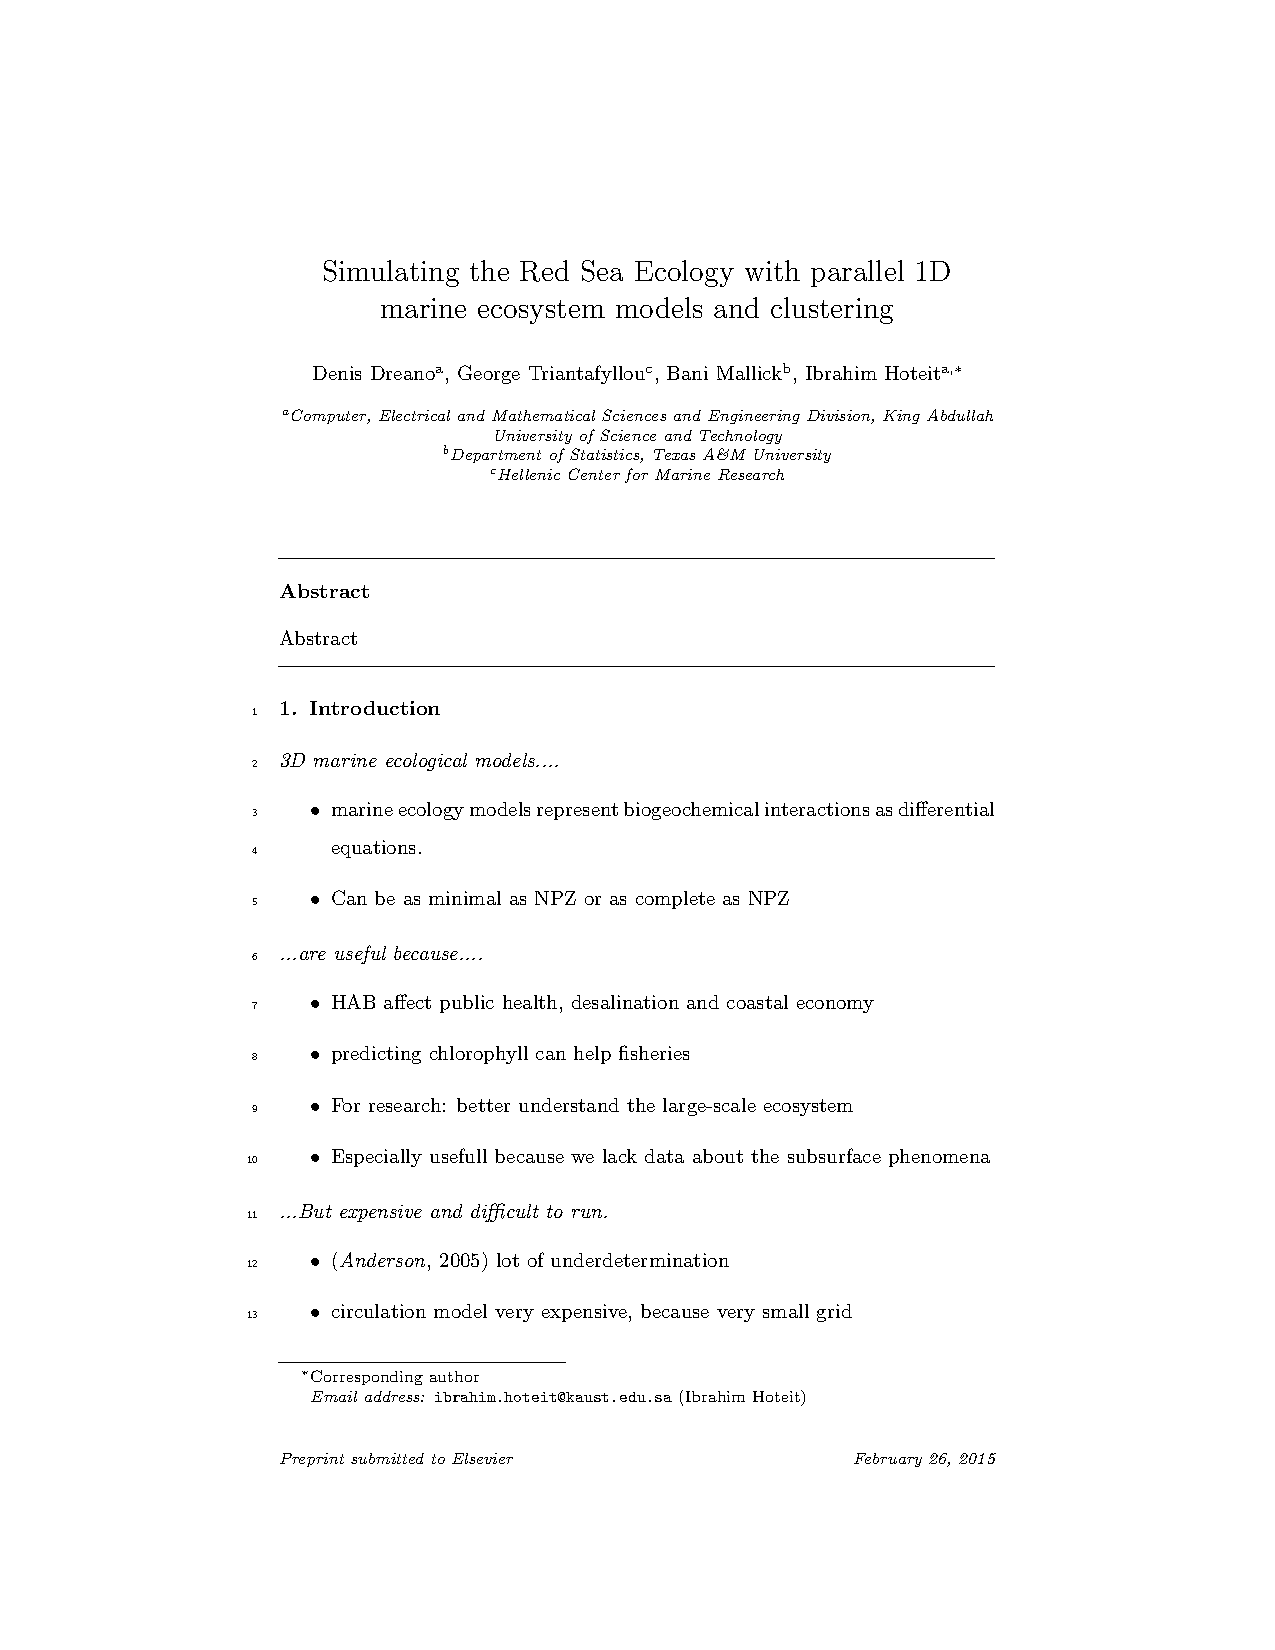
\includepdf[pages=-, pagecommand={}]{article.pdf}




\end{document}